\documentclass[a4paper,11pt]{article}
\usepackage[]{styles}
\usepackage[]{pgraphics}
\usepackage{amsmath}
\newcommand{\eqname}[1]{\tag*{#1}}% Tag equation with name

\newcommand\Rey{\mbox{\textit{Re}}}

\begin{document}

\maketitle

\newpage

\section{Equações Básicas}

\paragraph{} O campo magnético satisfaz $\mathbf{B} = \mu_0(\mathbf{M}+\mathbf{H})$. Seu divergente é nulo - $\nabla\cdot \mathbf{B} =  0$ -, indicação de que o campo é solenoidal, isto é: todas as linhas de campo magnético que saem da superfície têm de retornar a ela. Consequência dessas duas equações é


\begin{eqnarray}
\nabla\cdot \mathbf{M} = -\nabla\cdot\mathbf{H}	\label{mh1}
\end{eqnarray}


\paragraph{} Um pressuposto para nosso estudo atual é que trabalhos no regime magnetostático, o que rege $\nabla\times \mathbf{H} = \mathbf{0}$. Lembre-se que $\mathbf{H}$ é o fluxo elétrico; como este campo é irrotacional, temos que $\mathbf{H}$ é um campo potencial:

\begin{equation}
\mathbf{H} = -\nabla\phi \label{poth}	
\end{equation}

\paragraph{} De porte das Equações \ref{mh1} e \ref{poth}, obtém-se a equação de Poisson para a função potencial $\phi$ - apresentada na Equação \ref{eqcampomag}. Observação: uma malha quadrada $1\times 1$ será considerada para solução numérica.

\begin{align}
\nabla^2\phi &= \nabla\cdot \mathbf{M}\label{eqcampomag}\\ \eqname{Equação da Função Potencial}
\end{align}

\section{Condições de Contorno}
\paragraph{} Ora, não se pode resolver uma equação de Poisson sem condições de contorno. Com este intuito, lembremos que a componente normal de $\mathbf{B}$ deve ser contínua através da interface entre o meio de fora - considere meio 1, ar - e o de dentro - considere meio 2, fluido magnético -, isto é: $\left(\mathbf{B}_{\mathrm{f}} - \mathbf{B}_{\mathrm{d}}\right)\cdot \mathbf{n} = 0$. Com a ajuda da equação do campo magnético, obtém-se $\mu_0 (H_{\mathrm{f}}^{\mathrm{n}} + M_{\mathrm{f}}^{\mathrm{n}}) =  \mu_0(H_{\mathrm{d}}^{\mathrm{n}}+M_{\mathrm{d}}^{\mathrm{n}})$. No meio 1, não magnetizável, $M_f$ é nulo; utilizando a Equação \ref{poth}, obtêm-se as condições de contorno para nossa função potencial:

\begin{eqnarray}
\nabla\phi_{\mathrm{d}}^{\mathrm{n}} & = & -H_{\mathrm{f}}^{\mathrm{n}} + M_{\mathrm{d}}^{\mathrm{n}}
\end{eqnarray}

\paragraph{} Desenvolvendo a equação acima e utilizando os índices da malha escalonada - índices que variam entre 1 e $n$ na malha -, tem-se:

\begin{eqnarray}
\left.\frac{\partial \phi}{\partial x}\right|_{\mathrm{left}}\;\;&\approx&- H^{x}_{2,j} + M^{x}_{2,j}\\
\left.\frac{\partial \phi}{\partial x}\right|_{\mathrm{right}}&\approx&- H^{x}_{n,j} + M^{x}_{n,j}\\
\left.\frac{\partial \phi}{\partial y}\right|_{\mathrm{lower}}&\approx&- H^{y}_{i,2} + M^{y}_{i,2}\\
\left.\frac{\partial \phi}{\partial y}\right|_{\mathrm{upper}}&\approx&- H^{y}_{i,n} + M^{y}_{i,n}
\end{eqnarray}

\section{Problemas exemplo}
\paragraph{} Nesta seção, temos um campo magnético aplicado $\mathbf{H}$ e assume-se uma magnetização $\mathbf{M}$ do material dentro da cavidade para cada caso. Um detalhe importante é que a escolha de $\mathbf{H}$ e $\mathbf{M}$ não é arbitrária: é necessário que se satisfaça $\nabla\cdot \mathbf{B} = 0$.
\paragraph{} Foi utilizada uma malha $20\times 20$ e o valor máximo do divergente e do rotacional foi calculado.
\subsection{$\mathbf{M} = \mathbf{0}$ e $H_x = 1$}

\paragraph{} Veja Figuras \ref{p11}, \ref{p12} e \ref{p13}. Para este caso, tem-se: $\max \frac{1}{\mu_0}\nabla\cdot \mathbf{B}  = 7.19\cdot 10^{-13}$ e $\max \nabla\times \mathbf{H}  =1.97\cdot 	10^{-13}$


\begin{figure}[!ht]
\centering
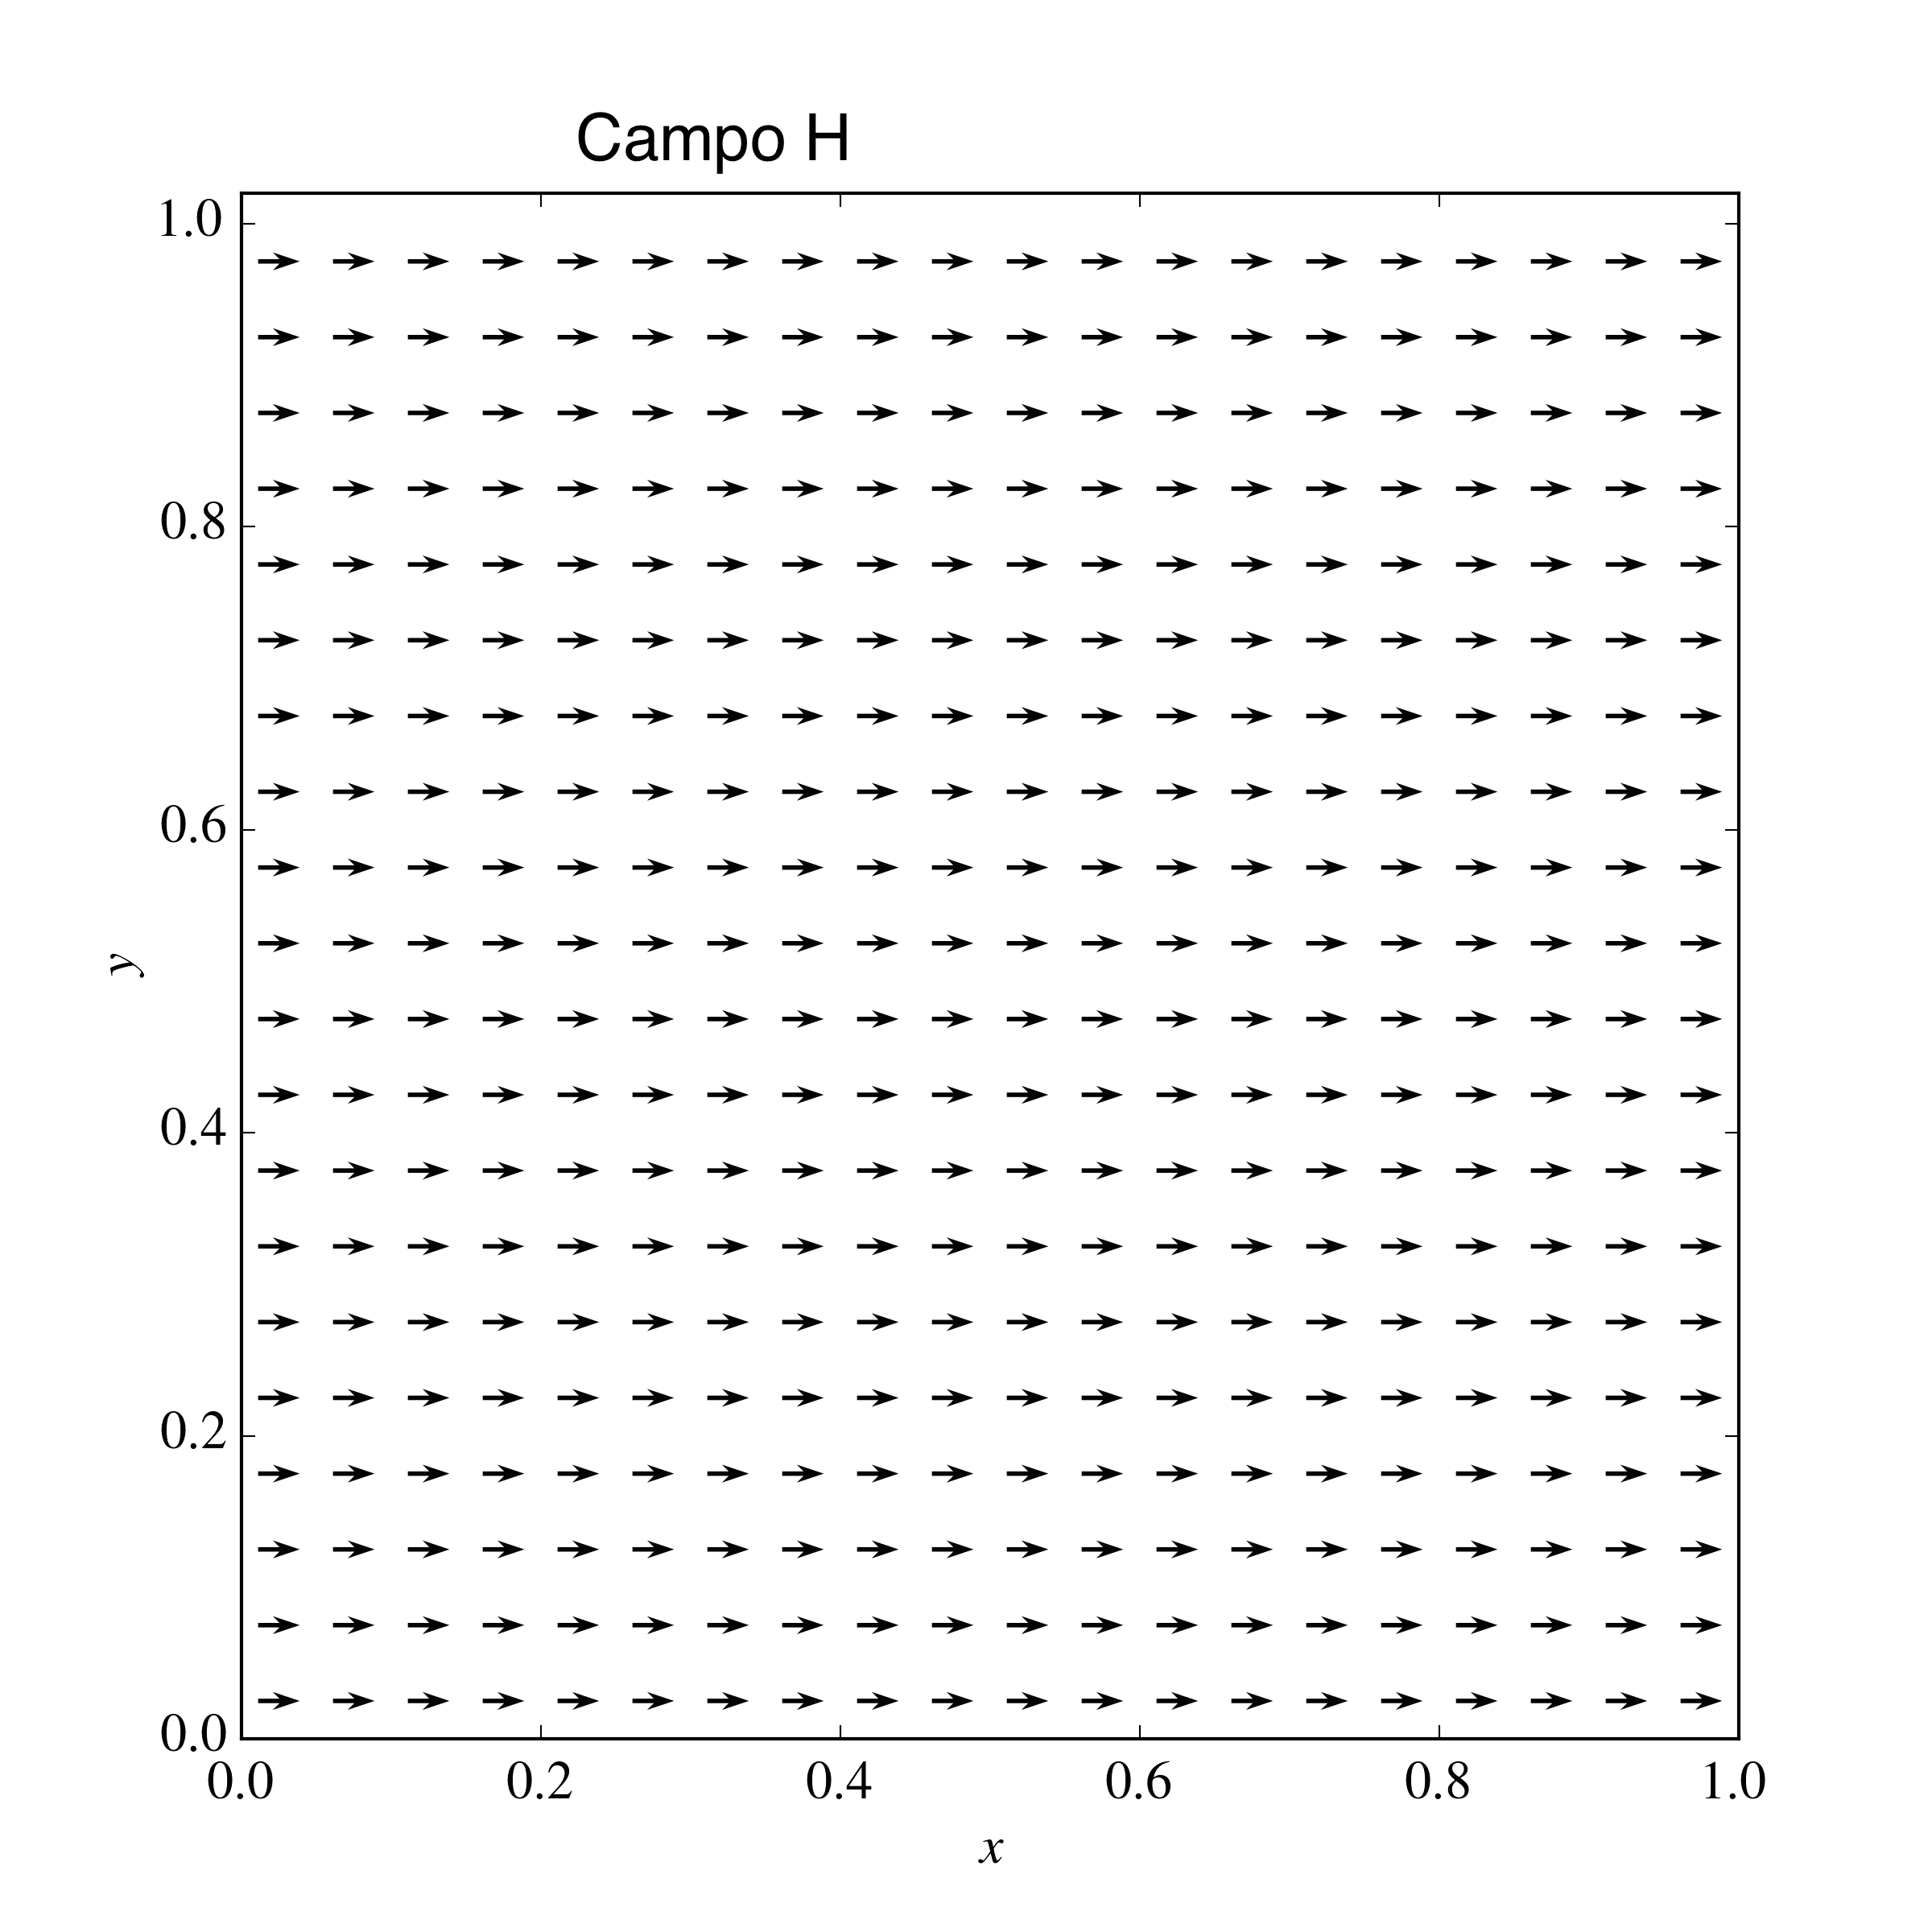
\includegraphics[width=10cm]{img/Hproblem0.png}
\caption{Campo vetorial $\mathbf{H}$ dentro da cavidade\label{p11}}
\end{figure}

\begin{figure}[!ht]
\centering
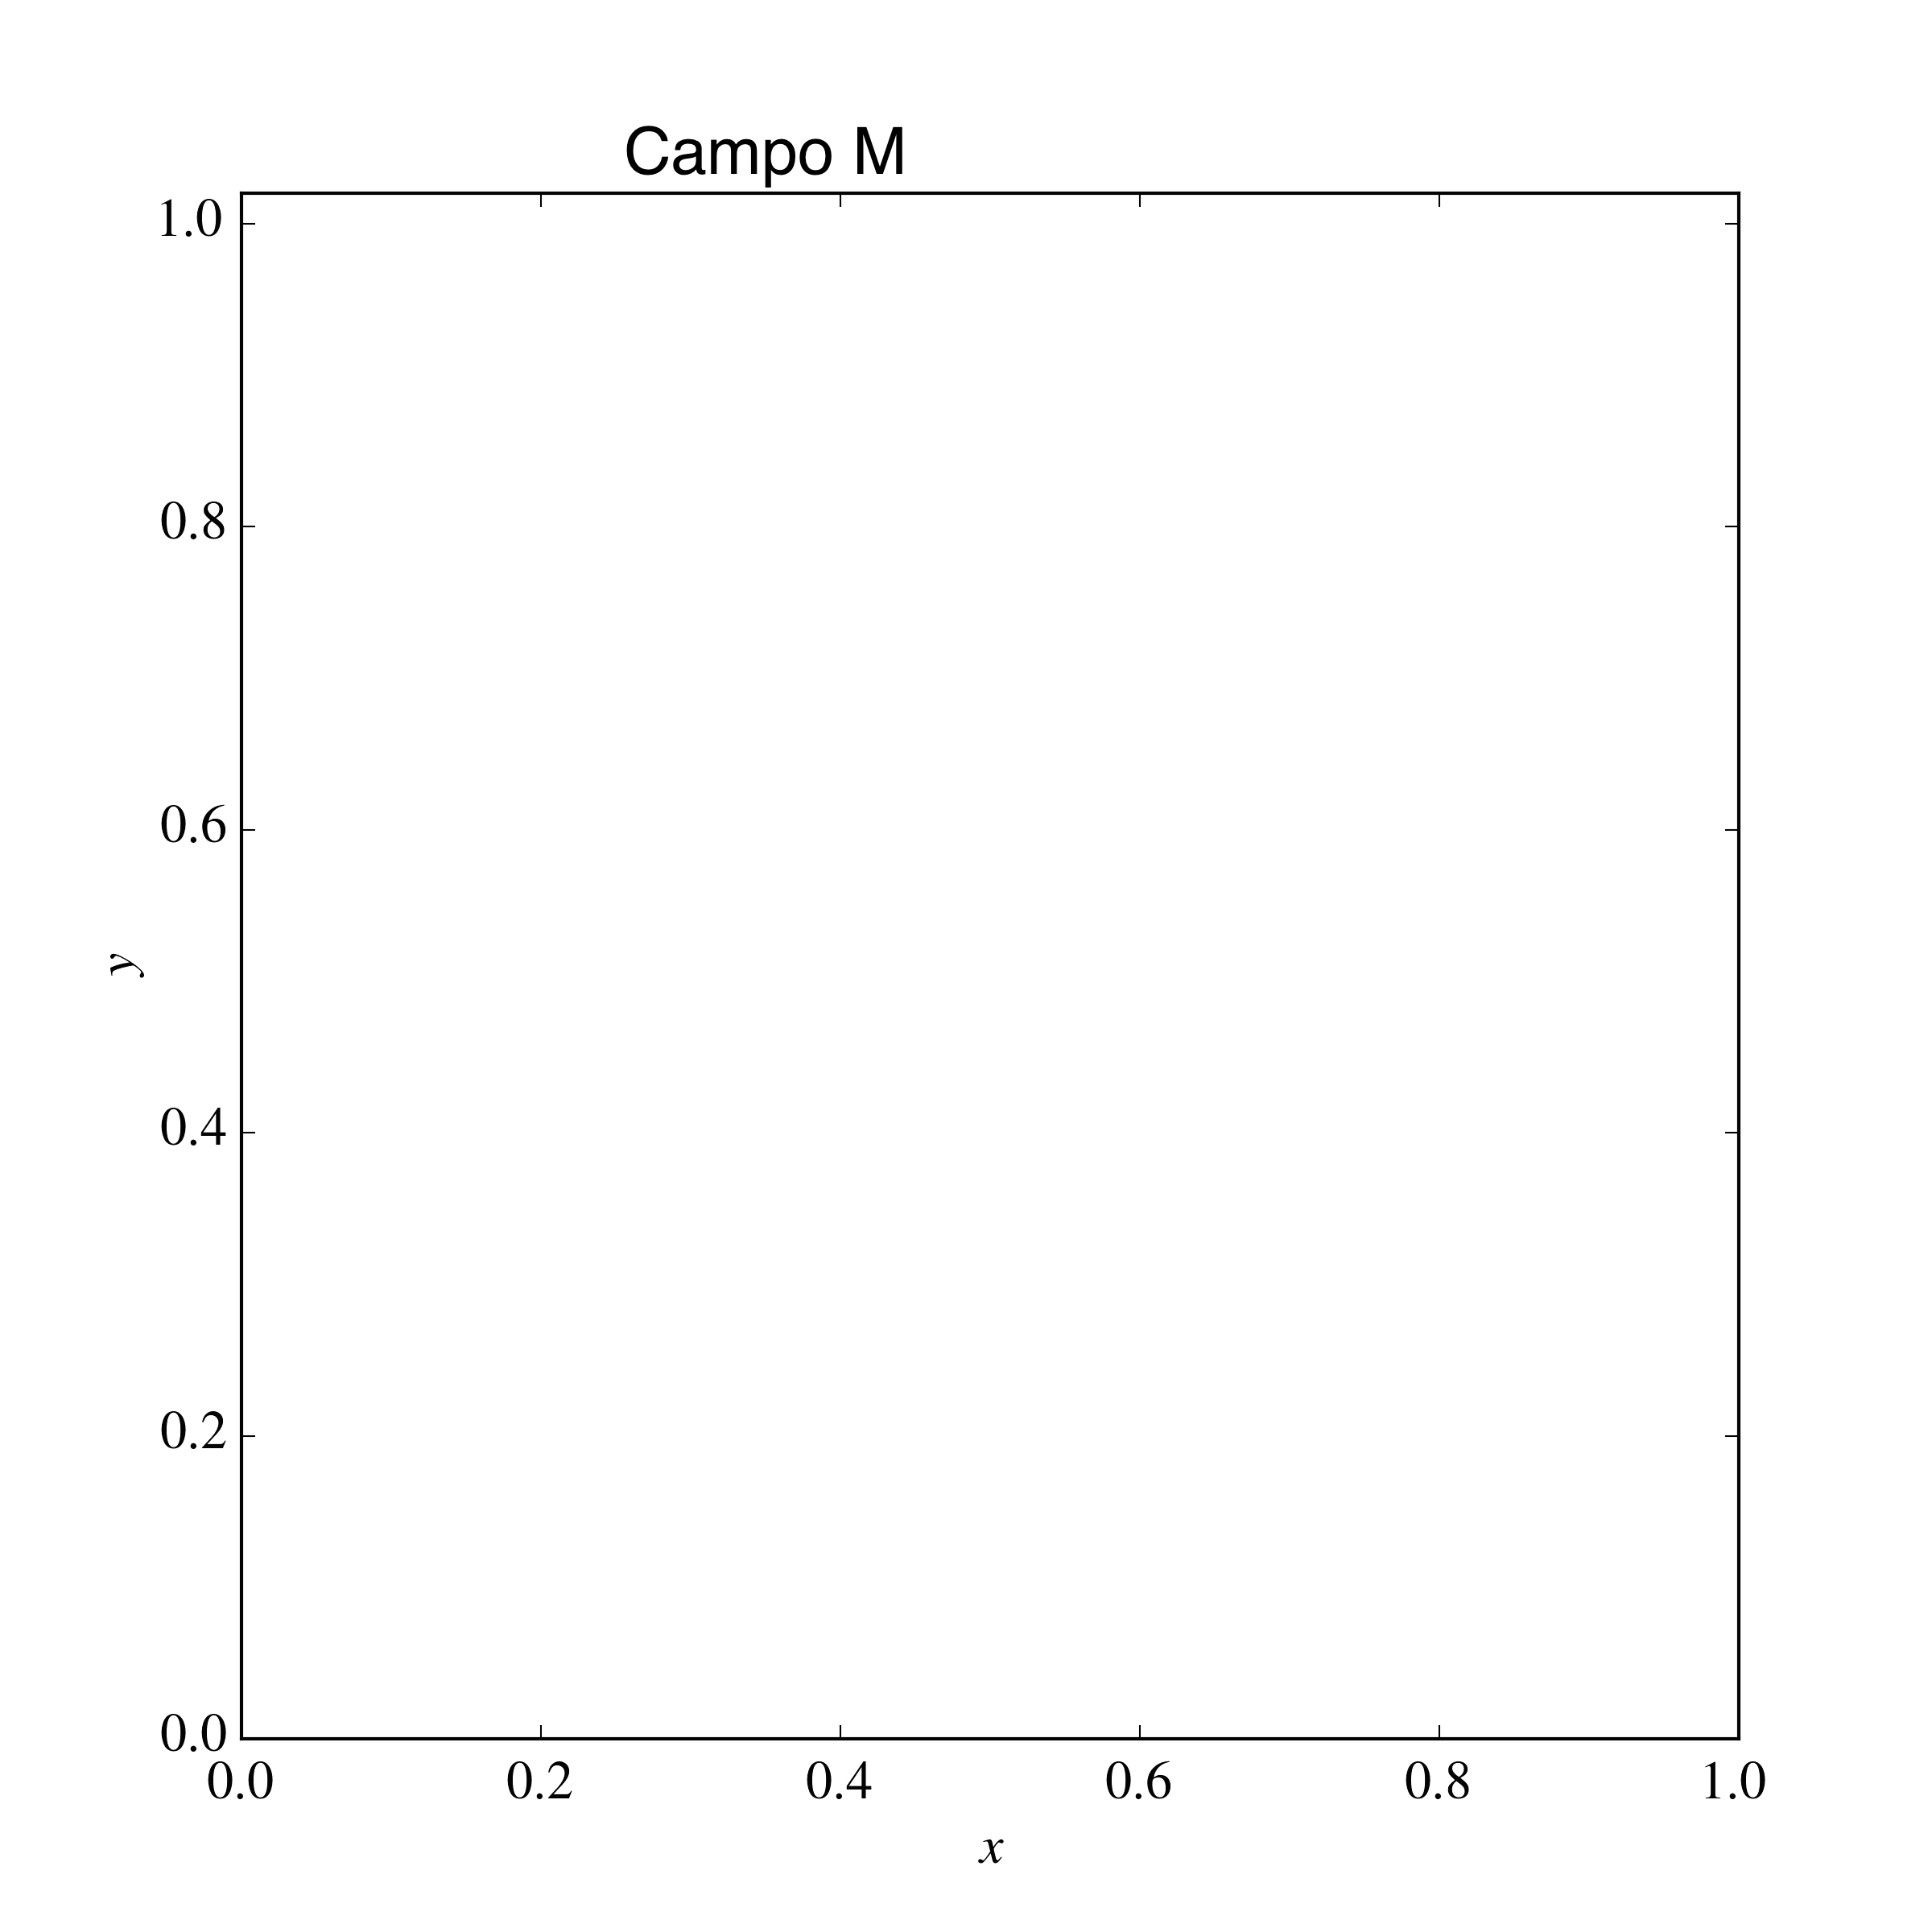
\includegraphics[width=10cm]{img/Mproblem0.png}
\caption{Campo vetorial $\mathbf{M}$ dentro da cavidade\label{p12}}
\end{figure}

\begin{figure}[!ht]
\centering
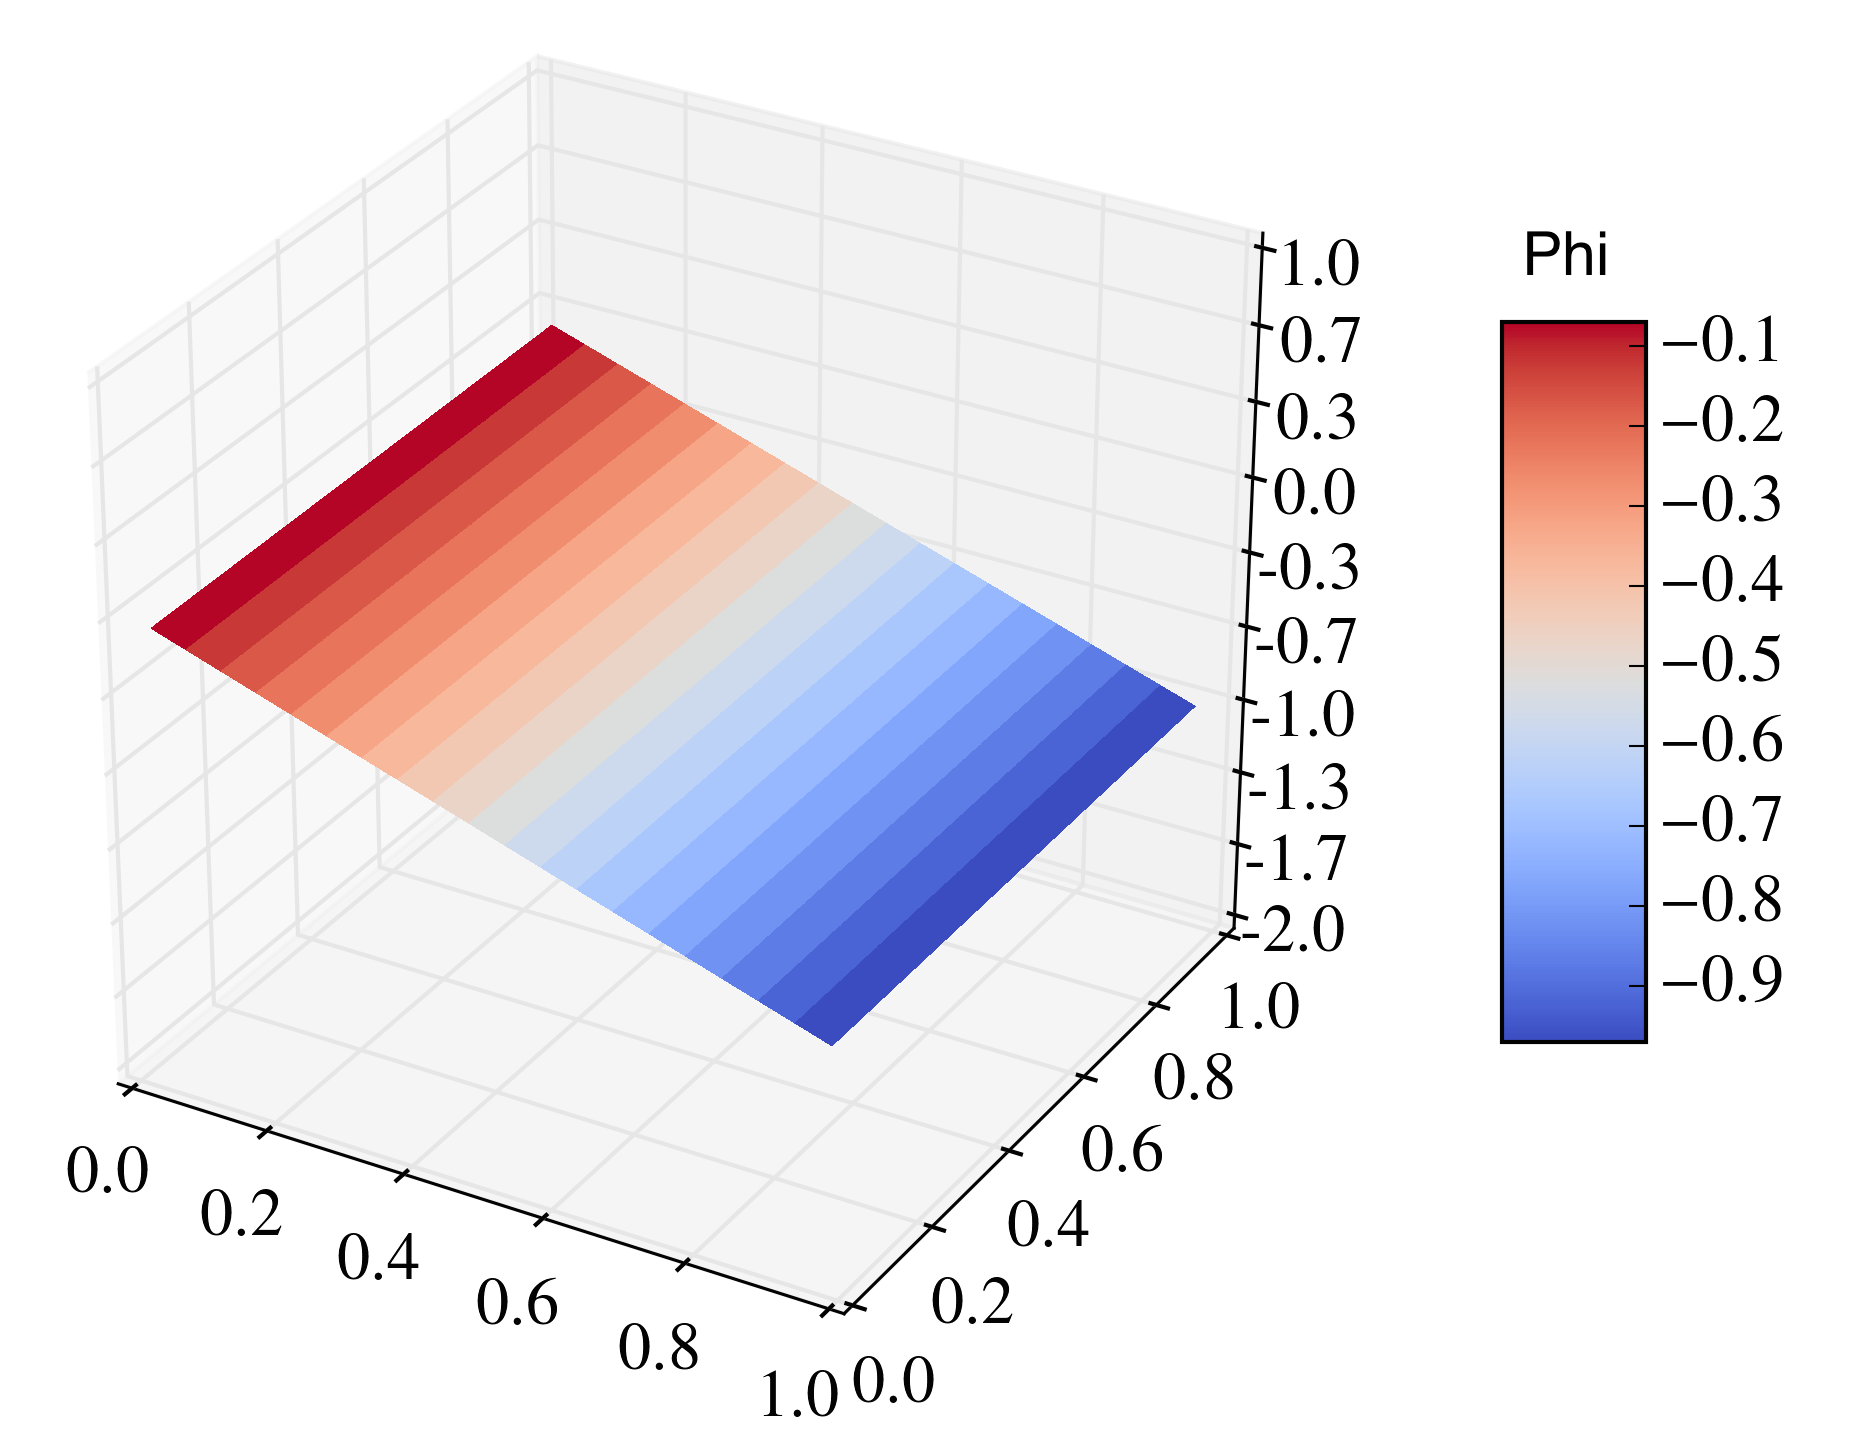
\includegraphics[width=10cm]{img/phiProblem0.png}
\caption{Função potencial $\phi$\label{p13}}
\end{figure}

\newpage
\subsection{$M_x = 0.1$ e $H_x = 1$}

\paragraph{} Veja Figuras \ref{p21}, \ref{p22} e \ref{p23}. Para este caso, tem-se: $\max \frac{1}{\mu_0}\nabla\cdot \mathbf{B}  = 6.62\cdot 10^{-13}$ e $\max \nabla\times \mathbf{H}  =1.78\cdot 	10^{-13}$


\begin{figure}[!ht]
\centering
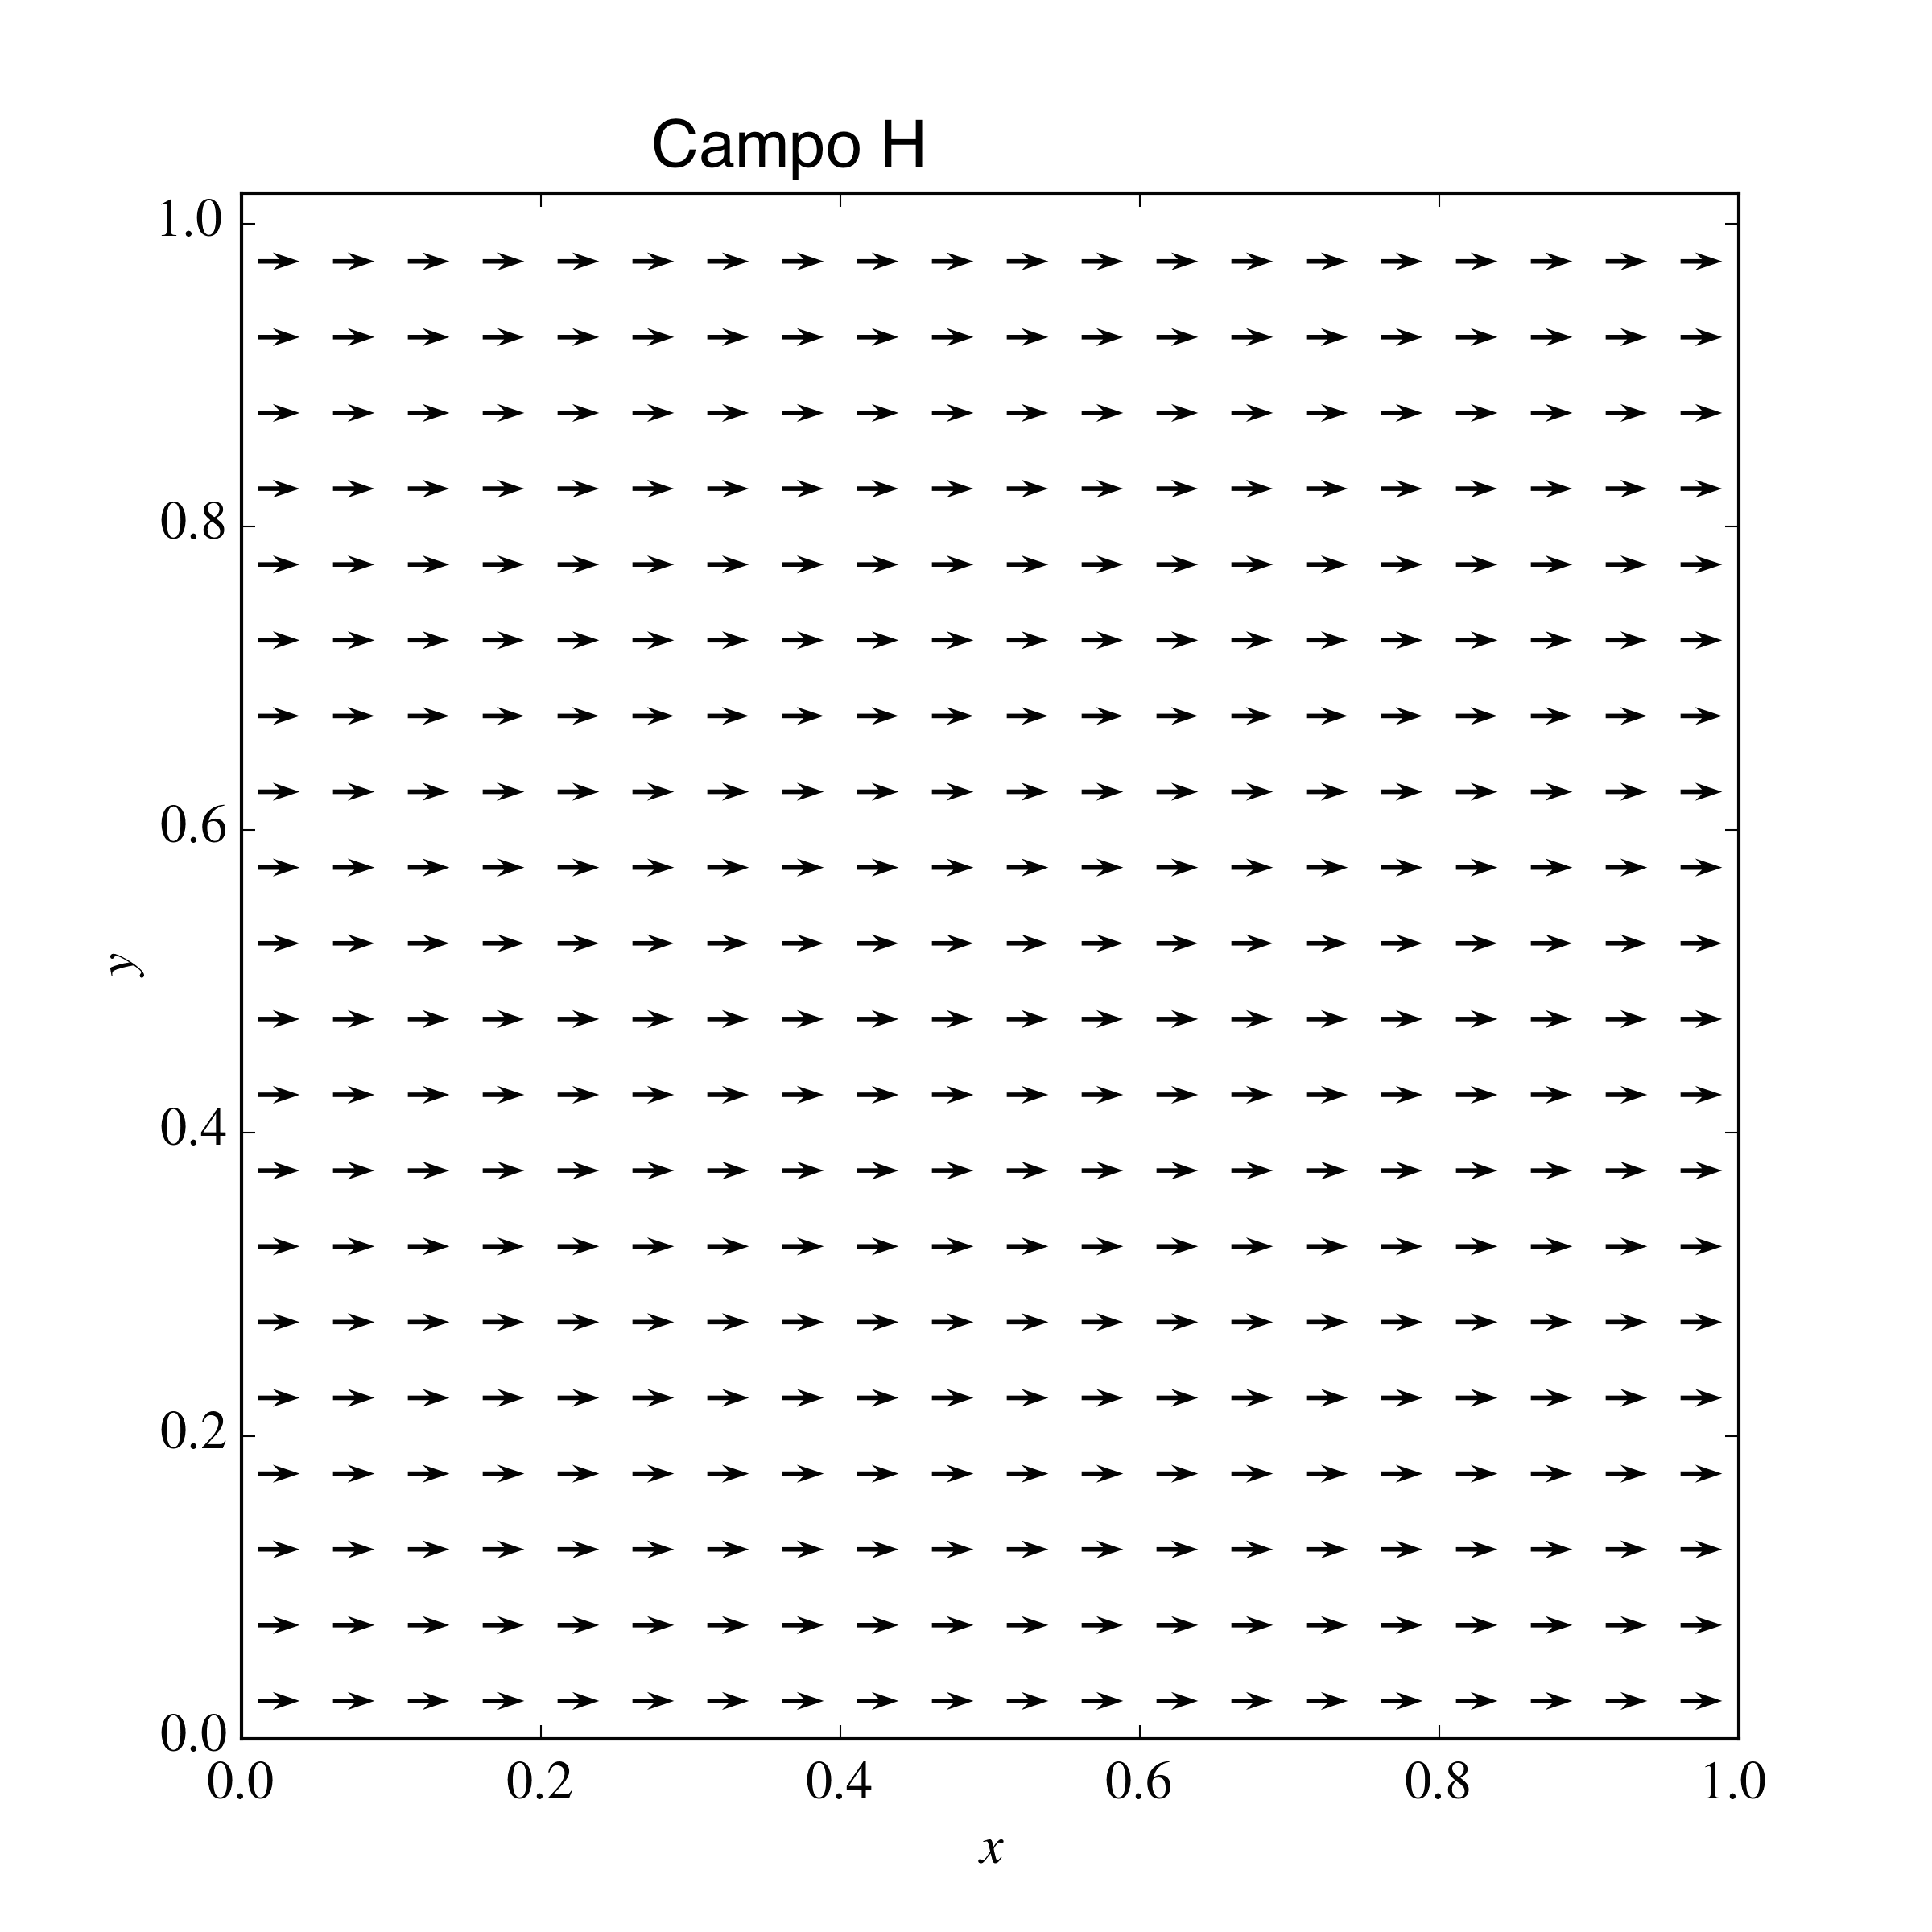
\includegraphics[width=10cm]{img/Hproblem1.png}
\caption{Campo vetorial $\mathbf{H}$ dentro da cavidade\label{p21}}
\end{figure}

\begin{figure}[!ht]
\centering
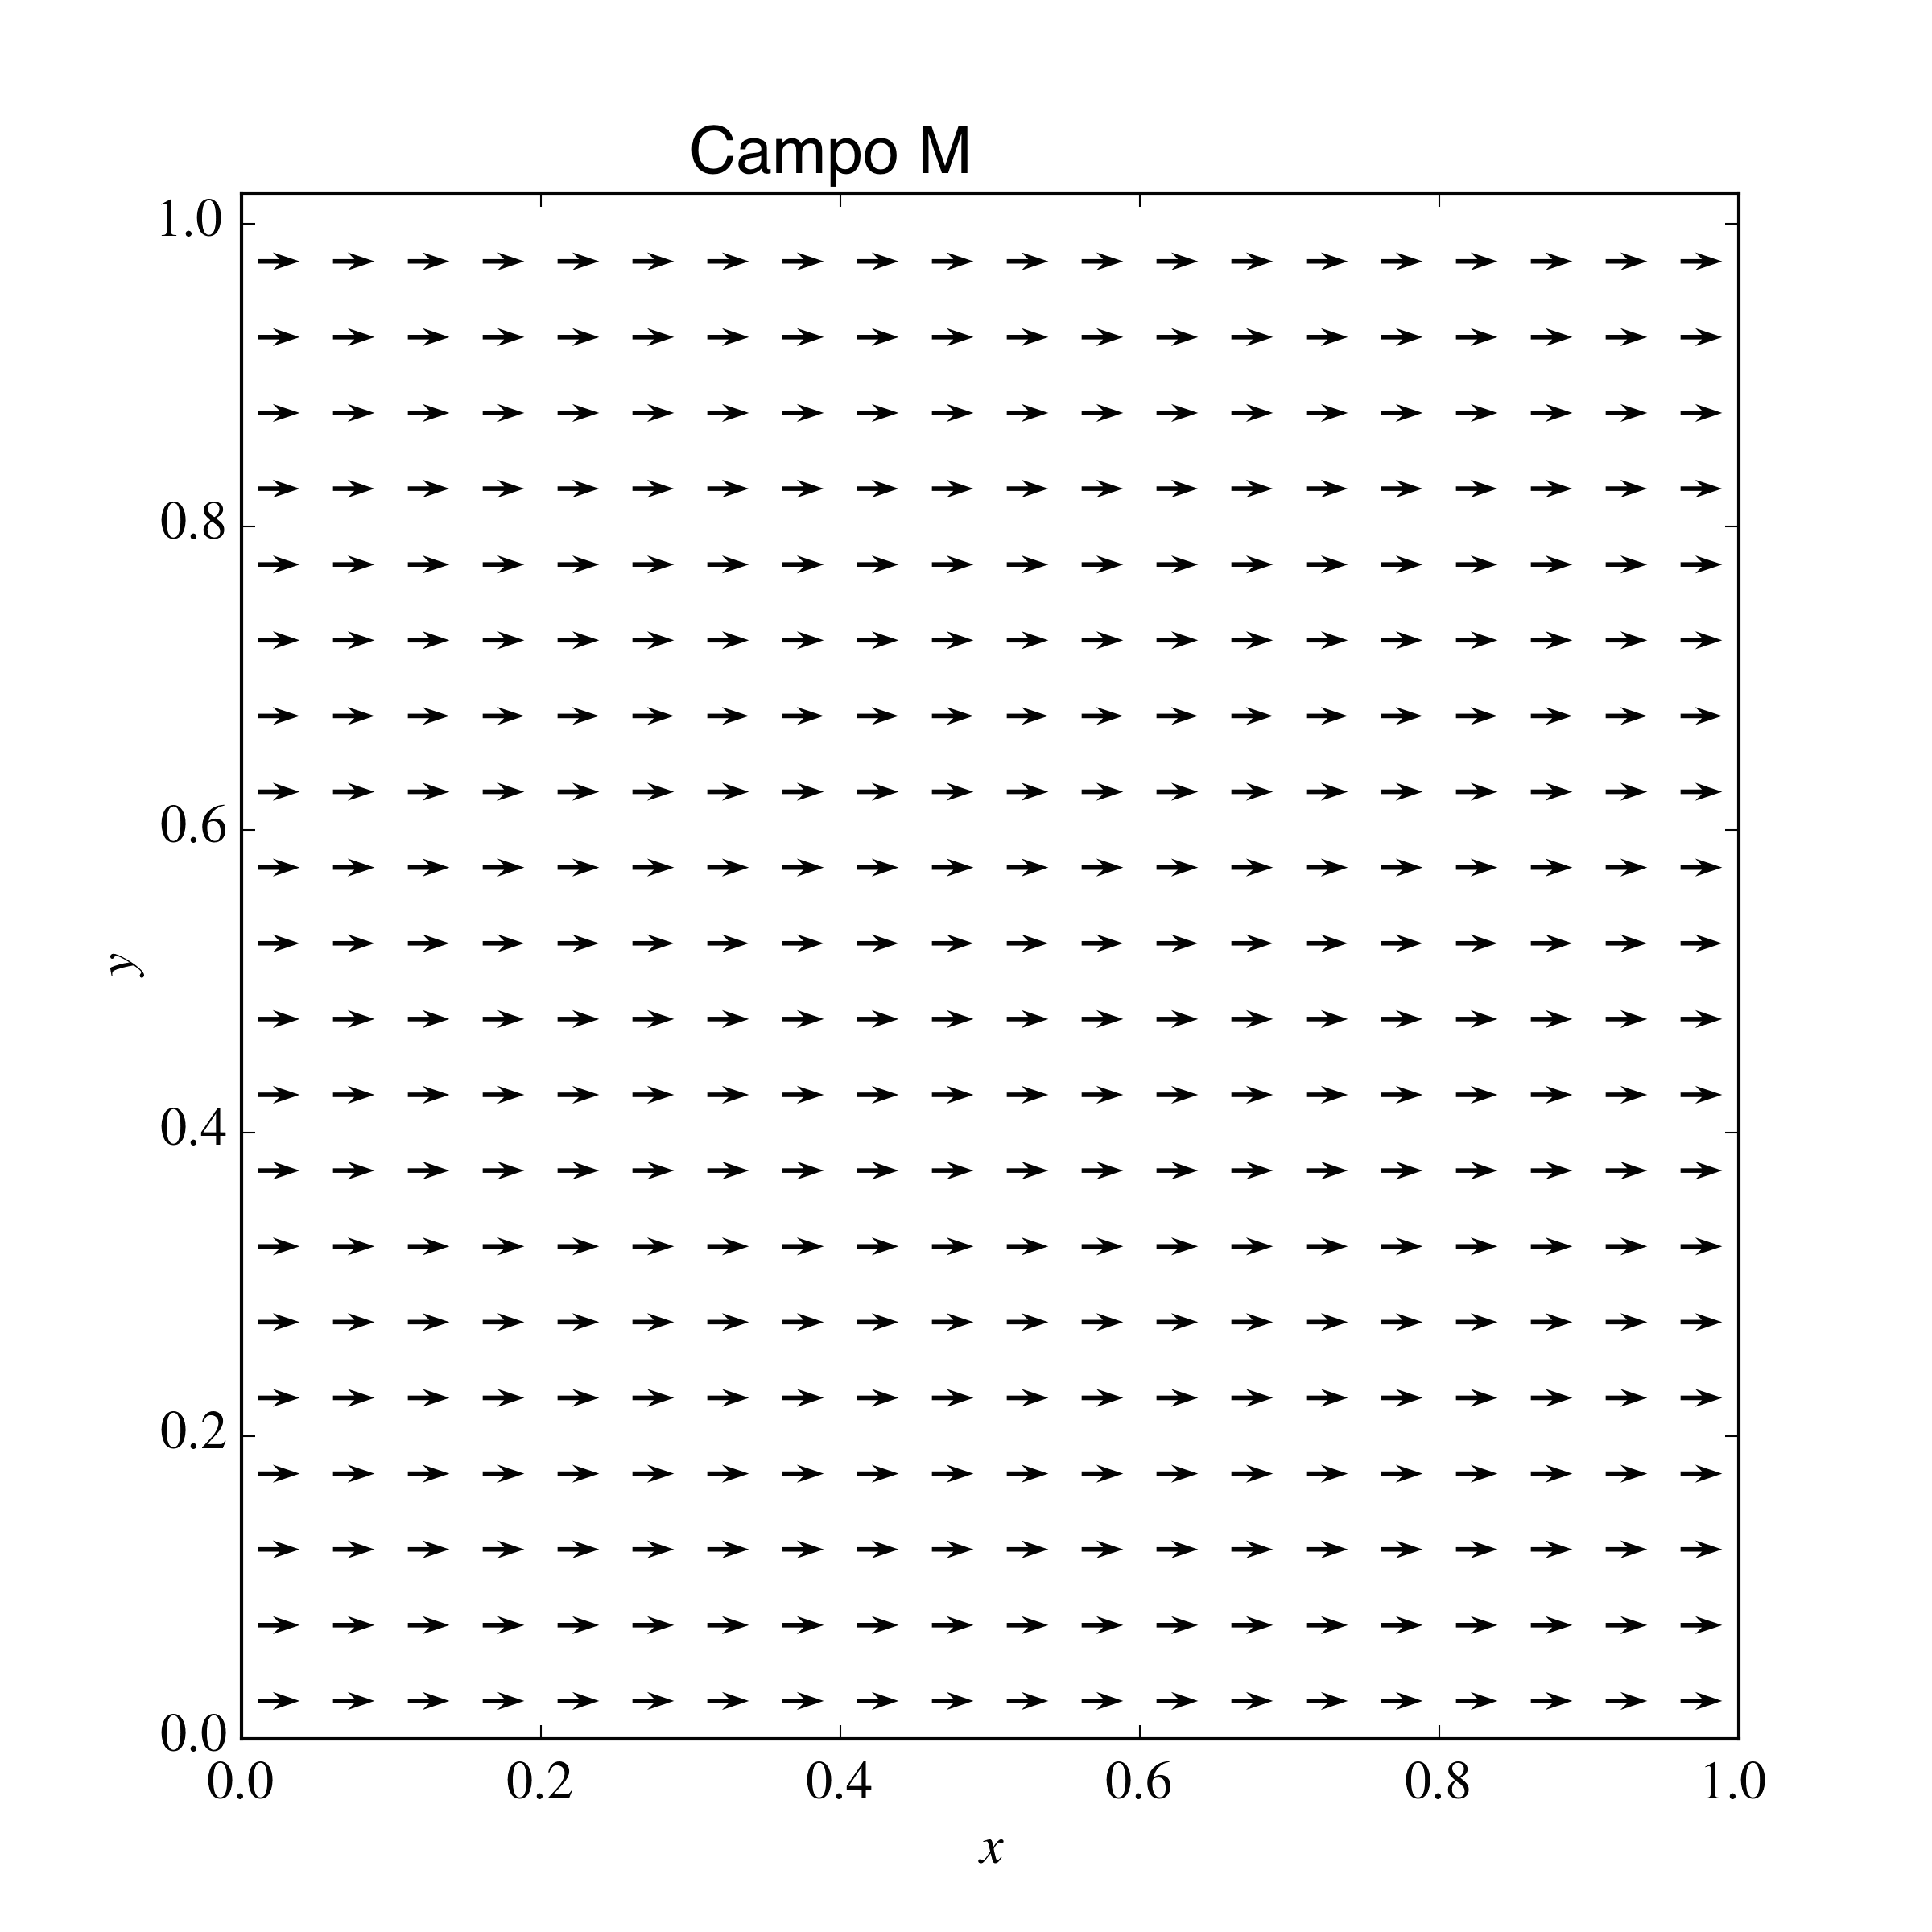
\includegraphics[width=10cm]{img/Mproblem1.png}
\caption{Campo vetorial $\mathbf{M}$ dentro da cavidade\label{p22}}
\end{figure}

\begin{figure}[!ht]
\centering
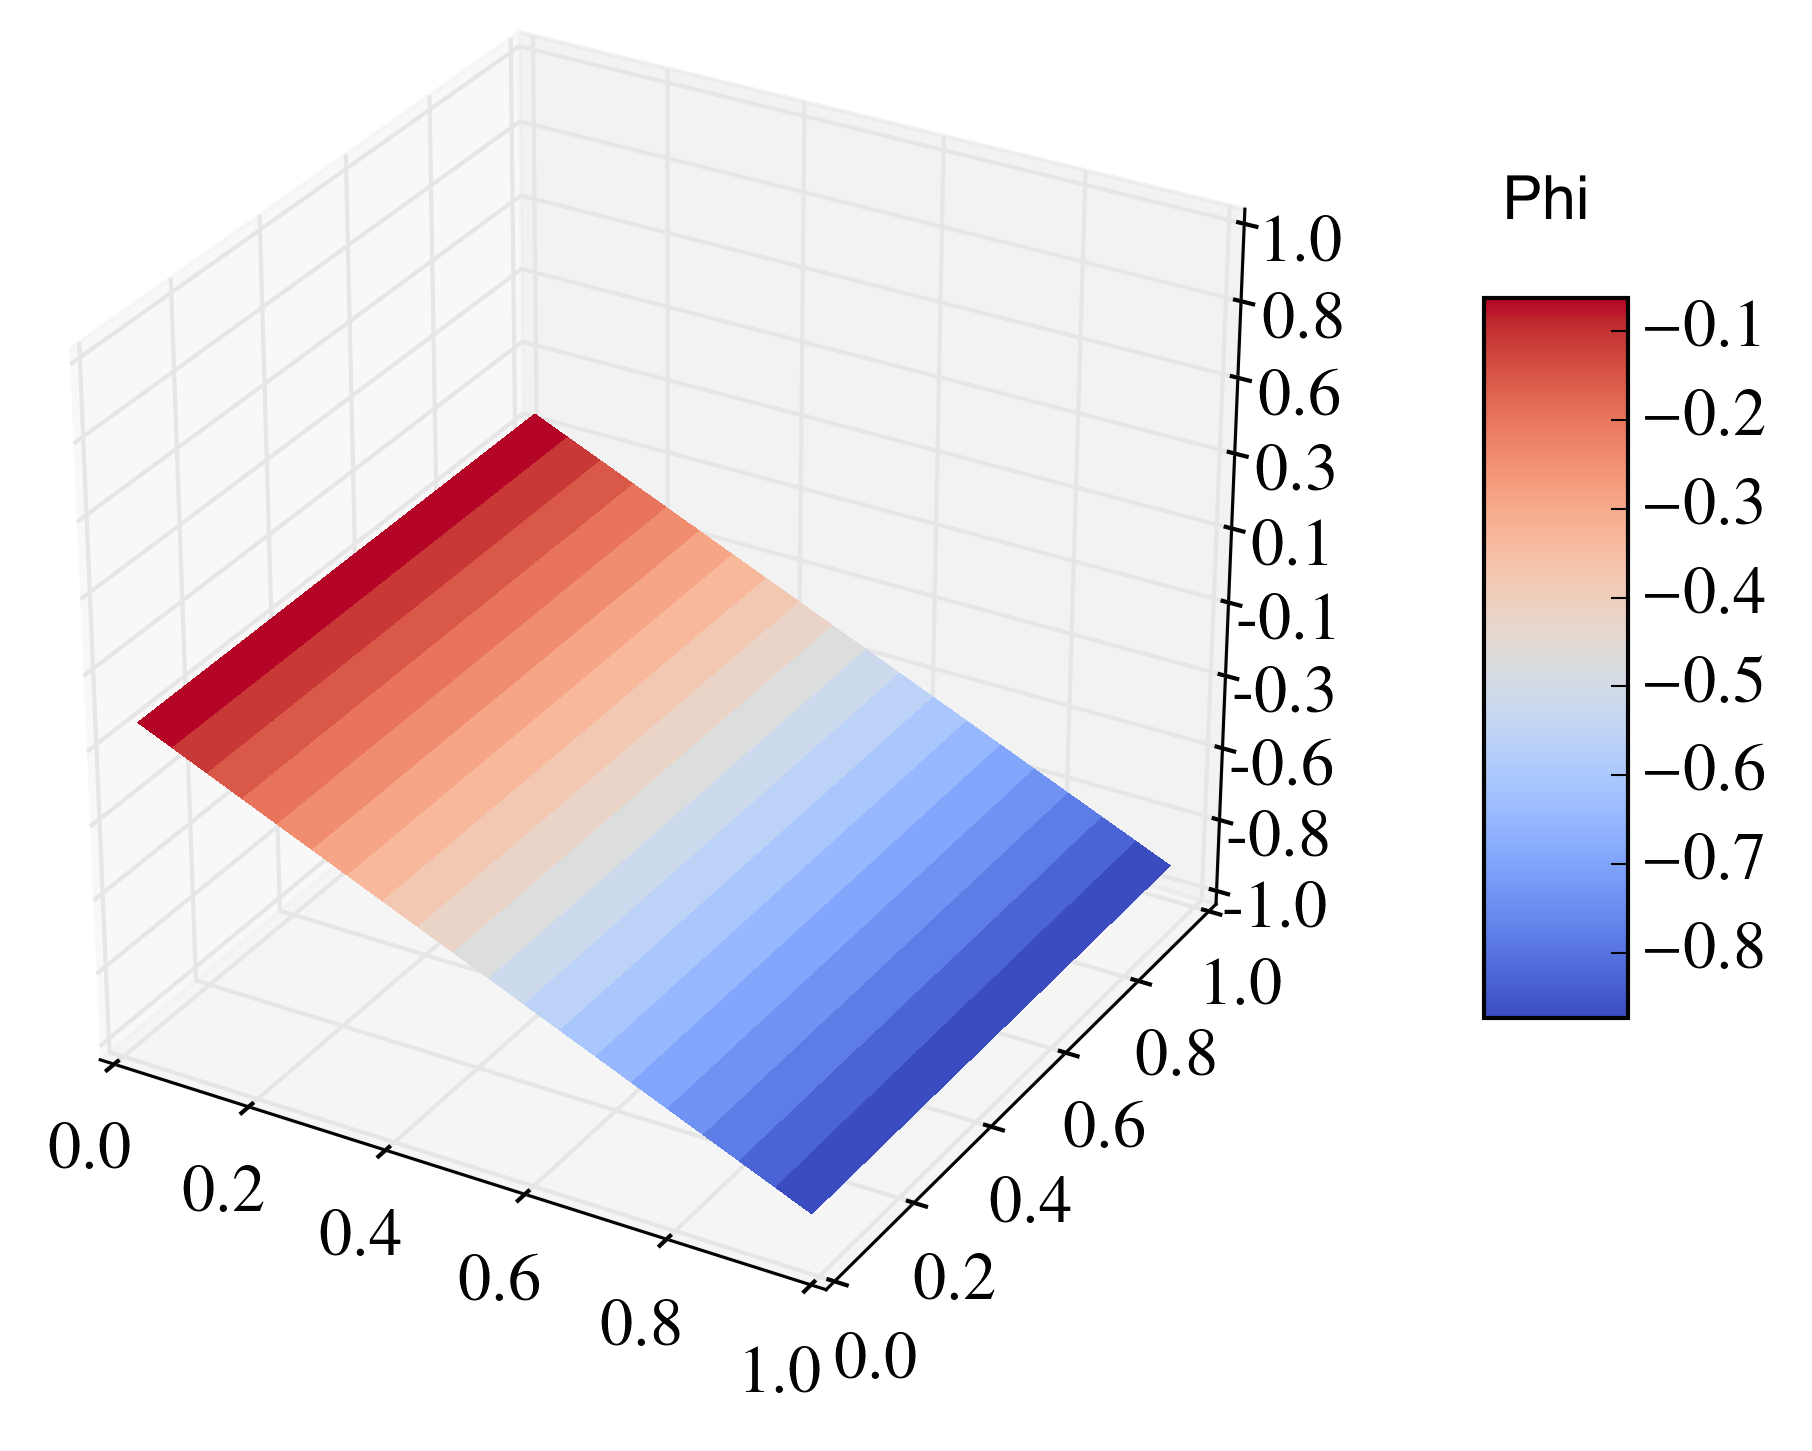
\includegraphics[width=10cm]{img/phiProblem1.png}
\caption{Função potencial $\phi$\label{p23}}
\end{figure}


\newpage
\subsection{$\mathbf{M} = 0.1(\mathbf{i}+\mathbf{j})$ e $H_x = 1$}
\paragraph{} Veja Figuras \ref{p31}, \ref{p32} e \ref{p33}. Para este caso, tem-se: $\max \frac{1}{\mu_0}\nabla\cdot \mathbf{B}  = 5.59\cdot 10^{-13}$ e $\max \nabla\times \mathbf{H}  =1.51\cdot 	10^{-13}$

\begin{figure}[!ht]
\centering
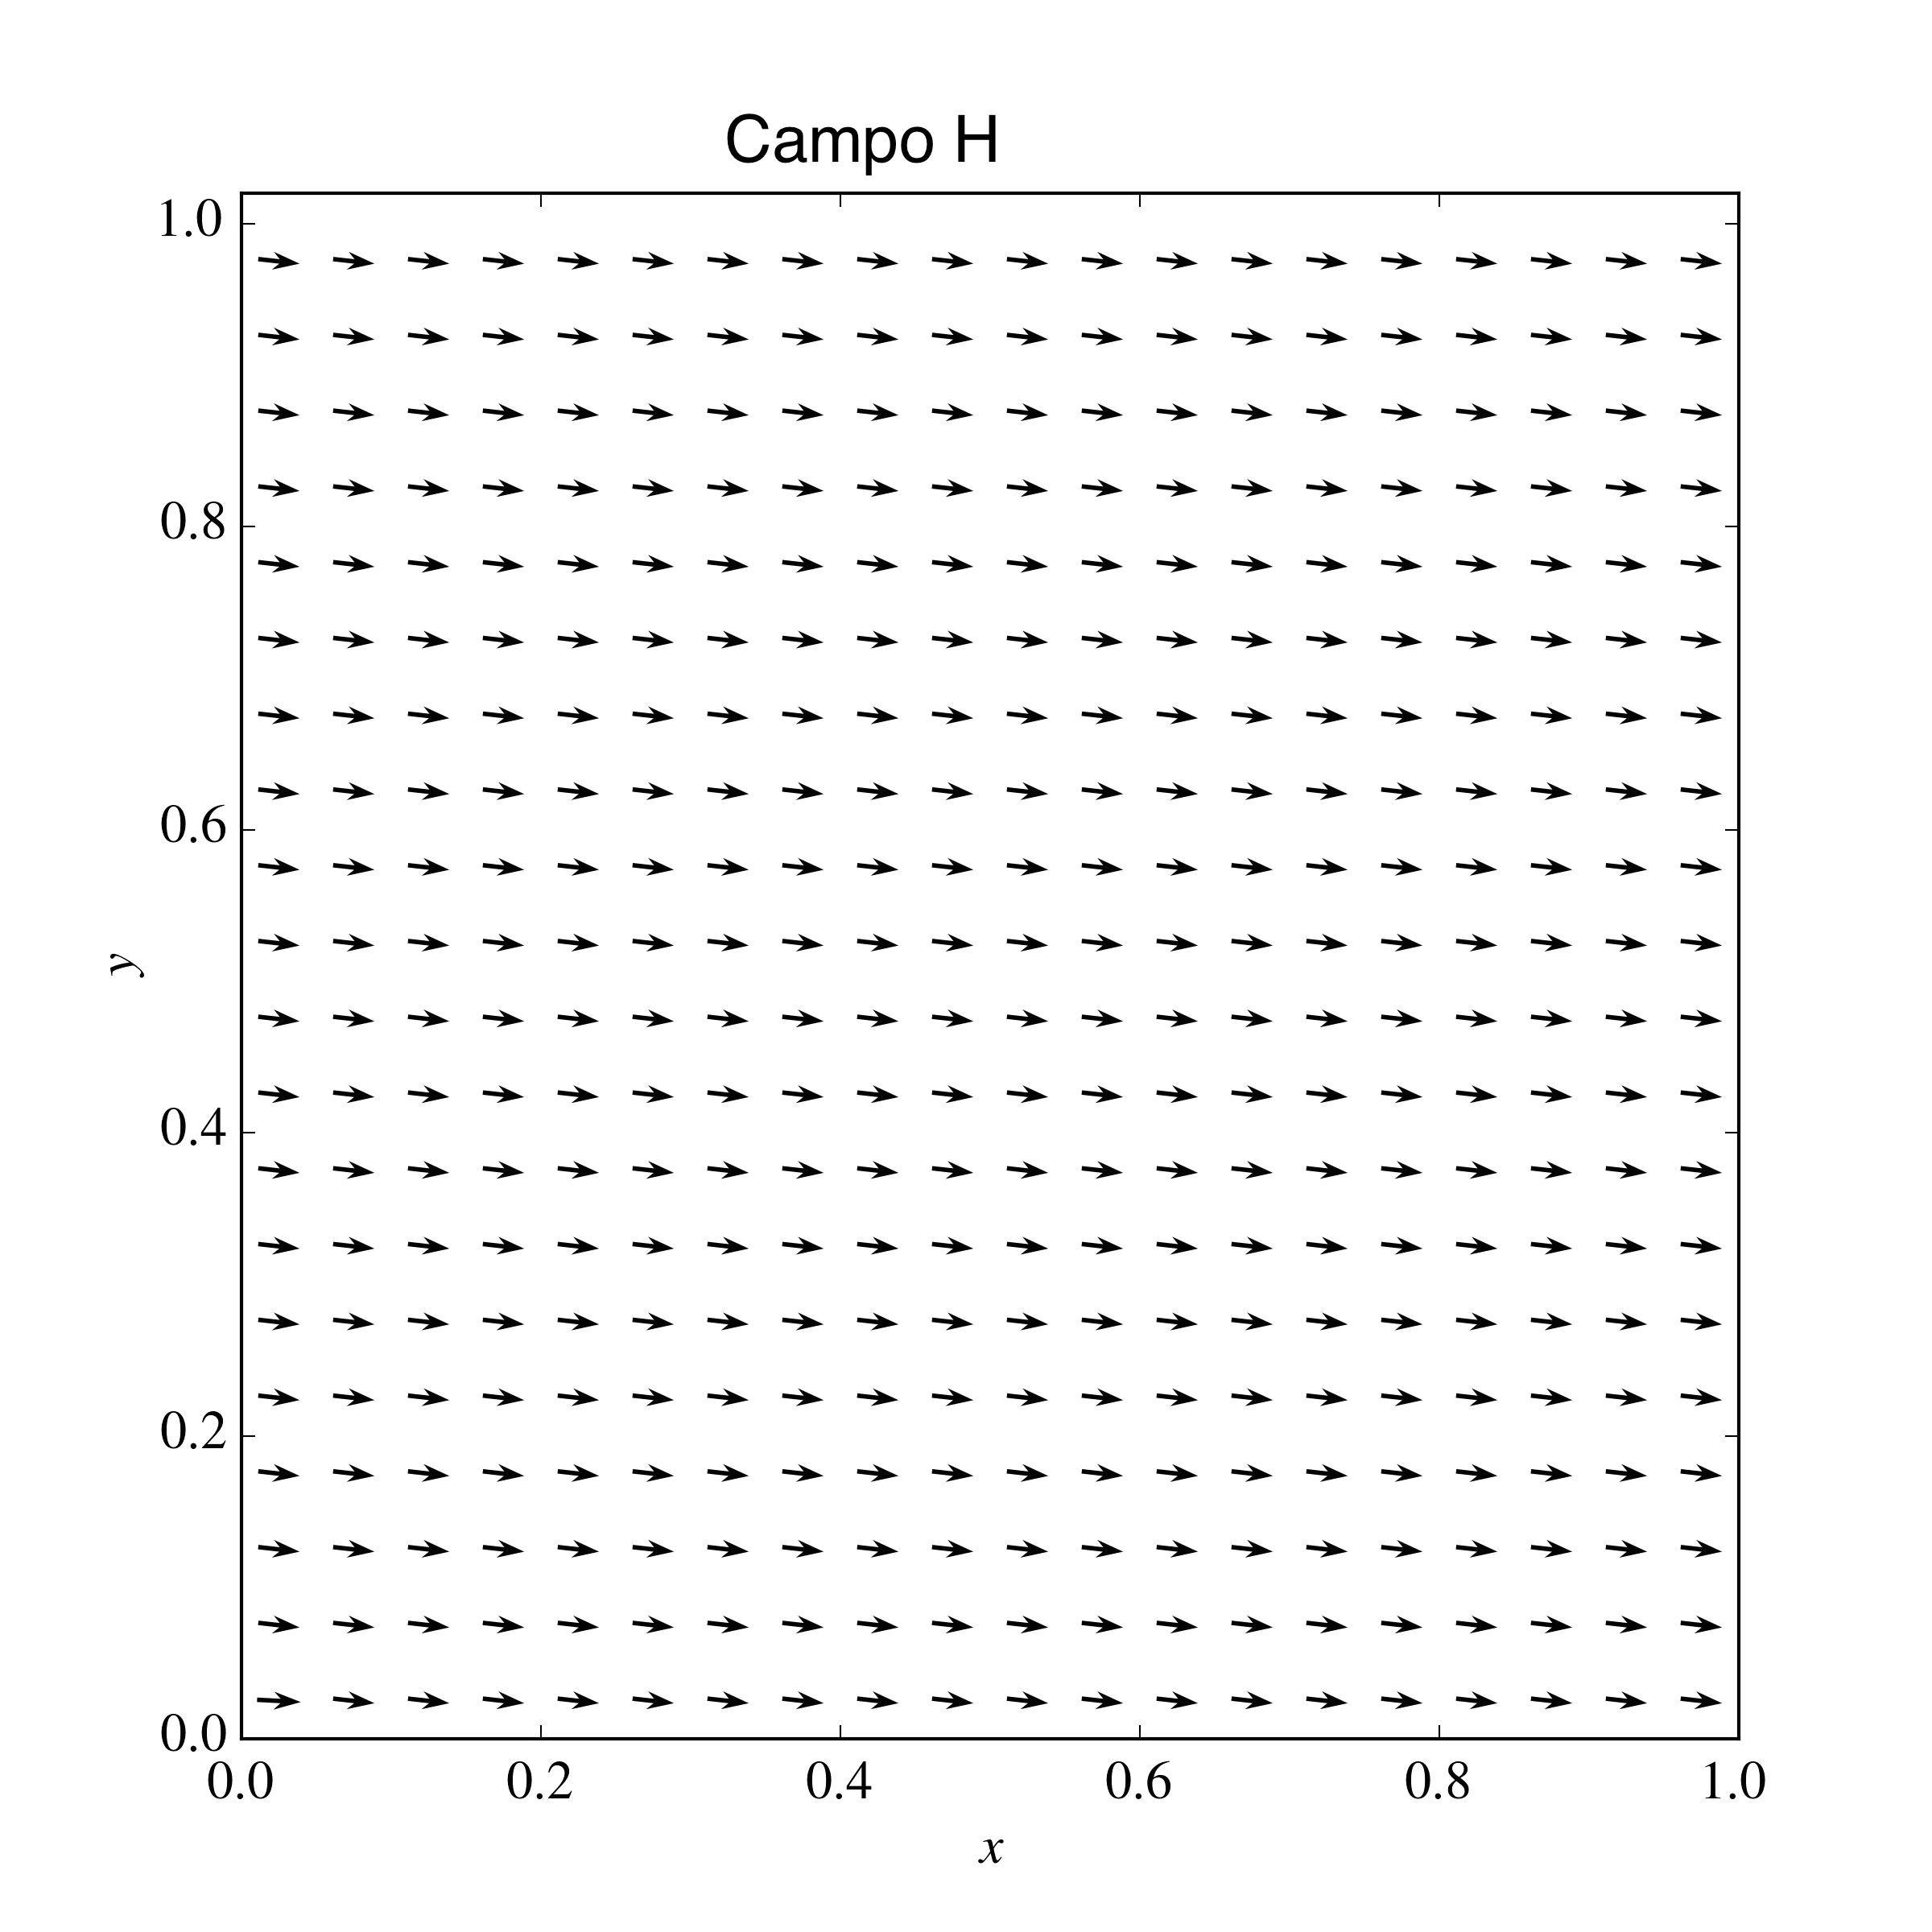
\includegraphics[width=10cm]{img/Hproblem2.png}
\caption{Campo vetorial $\mathbf{H}$ dentro da cavidade\label{p31}}
\end{figure}

\begin{figure}[!ht]
\centering
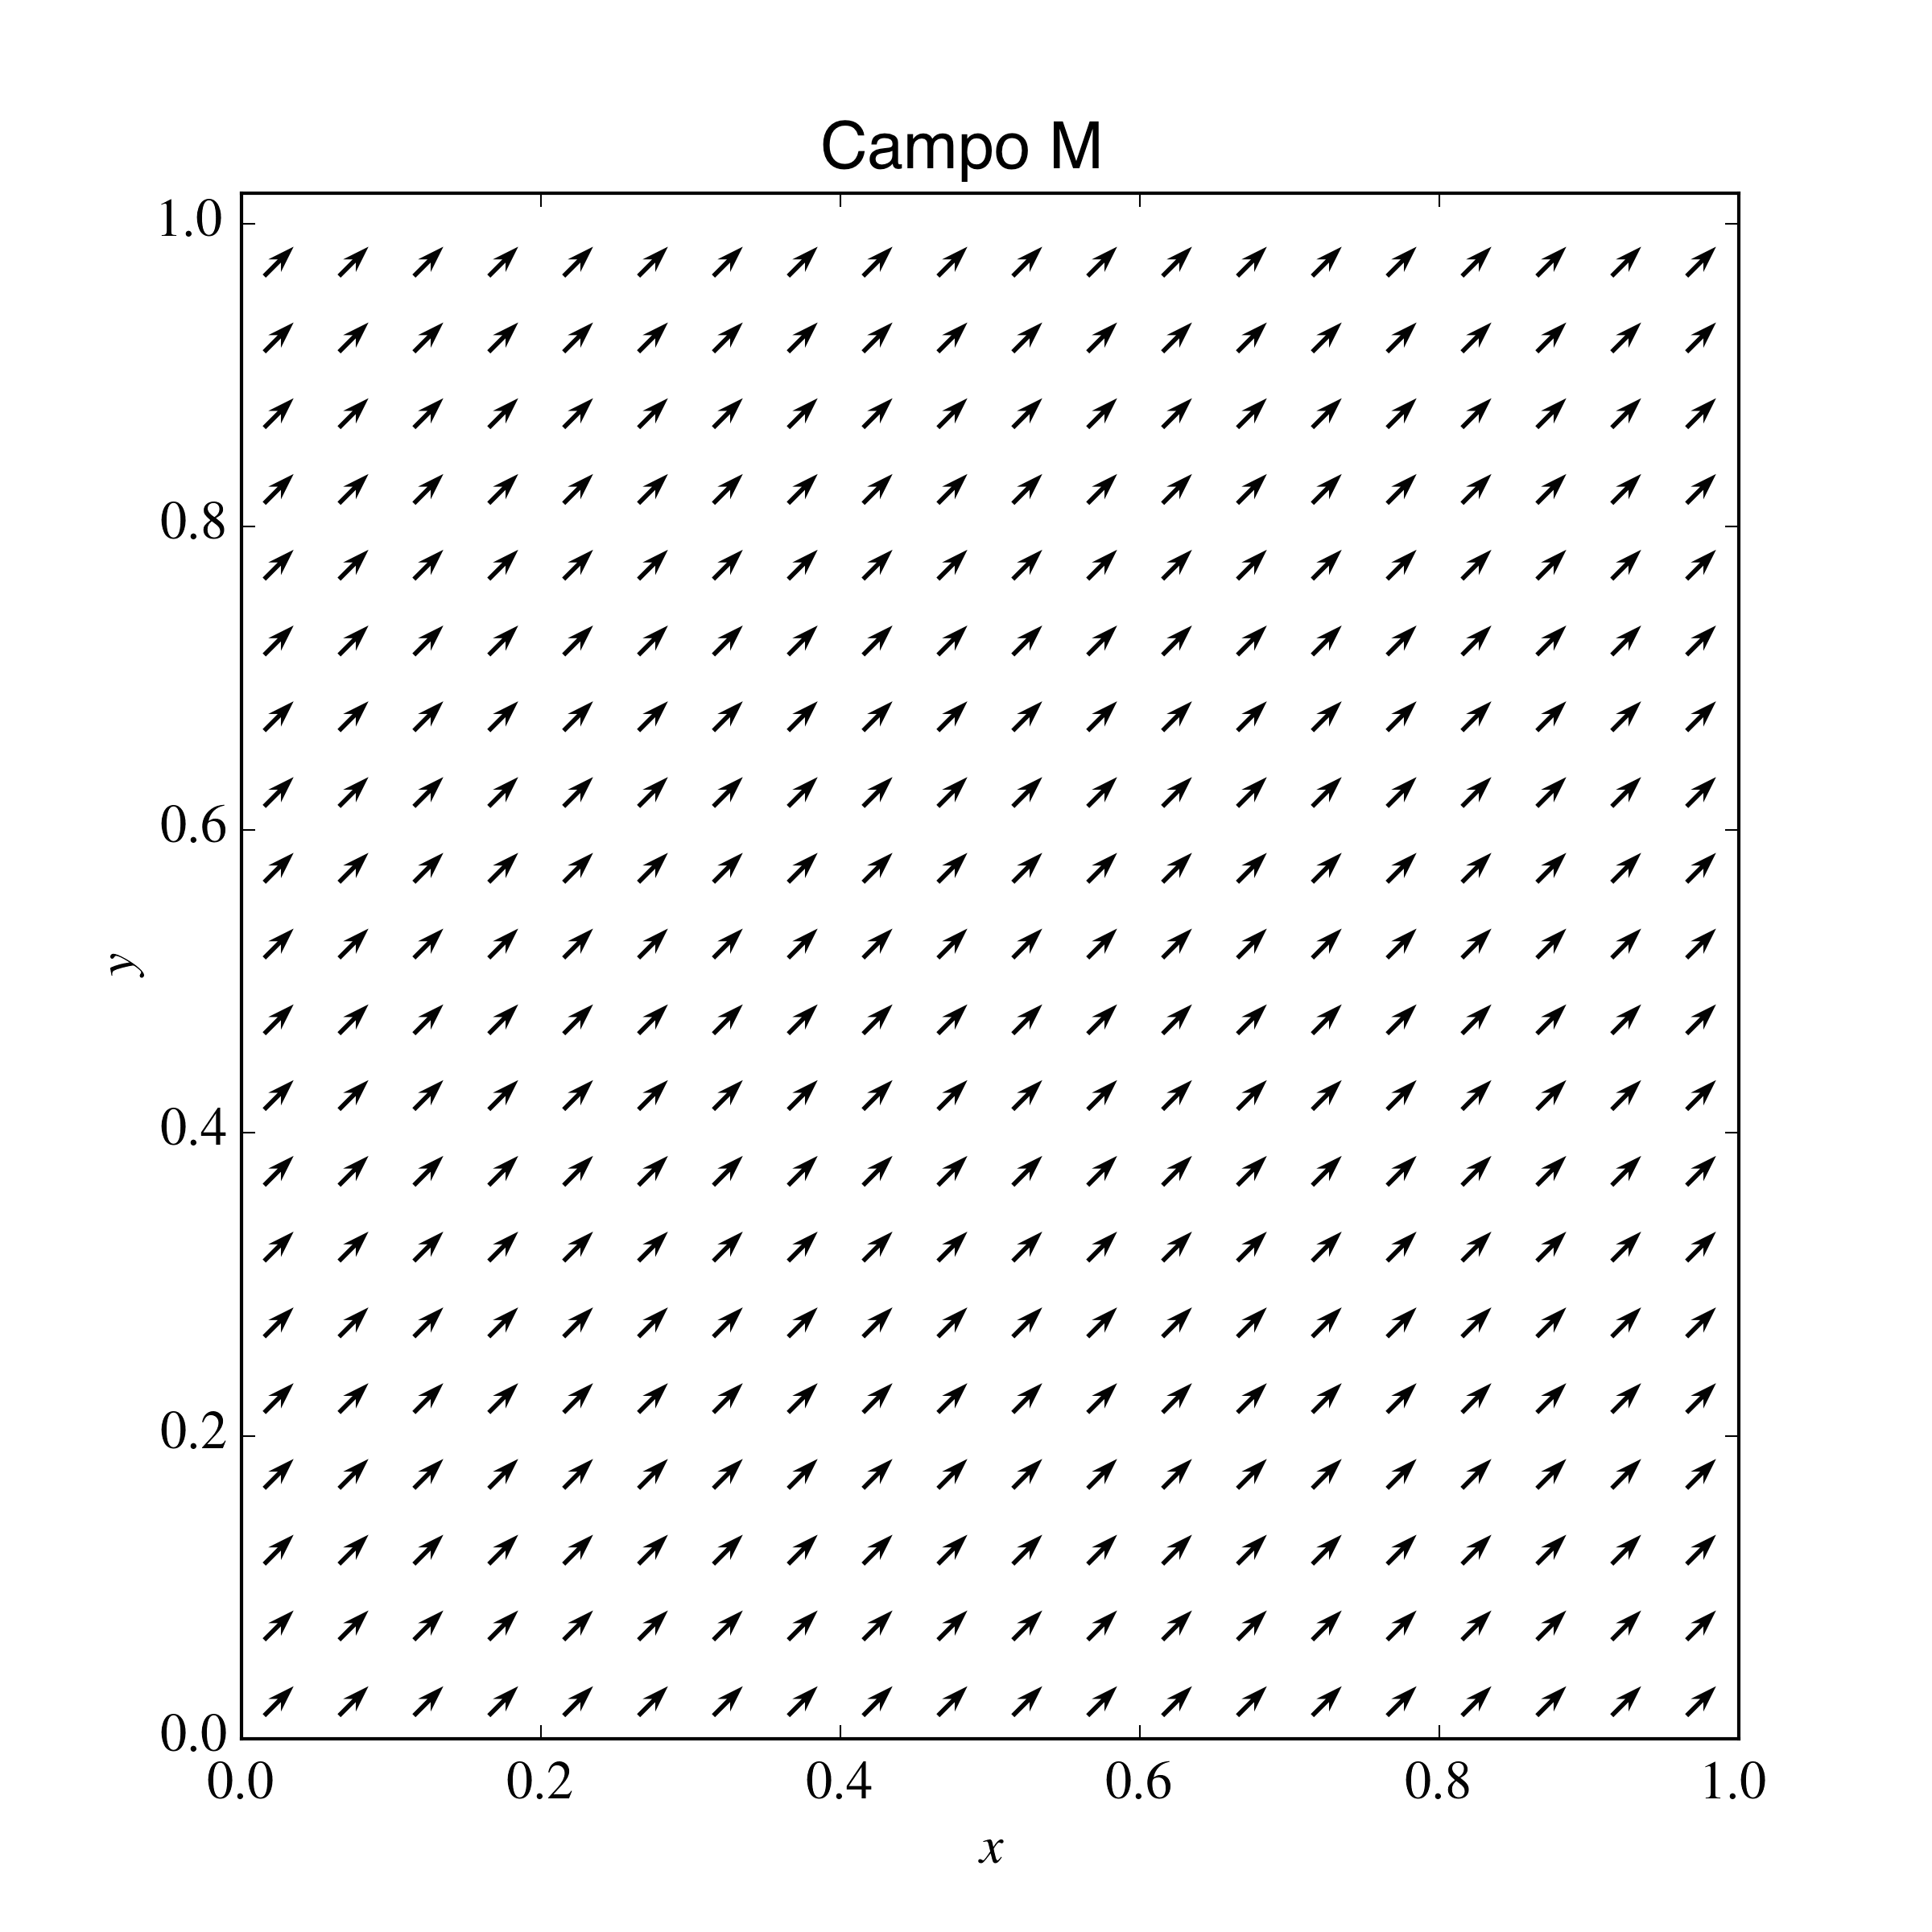
\includegraphics[width=10cm]{img/Mproblem2.png}
\caption{Campo vetorial $\mathbf{M}$ dentro da cavidade\label{p32}}
\end{figure}

\begin{figure}[!ht]
\centering
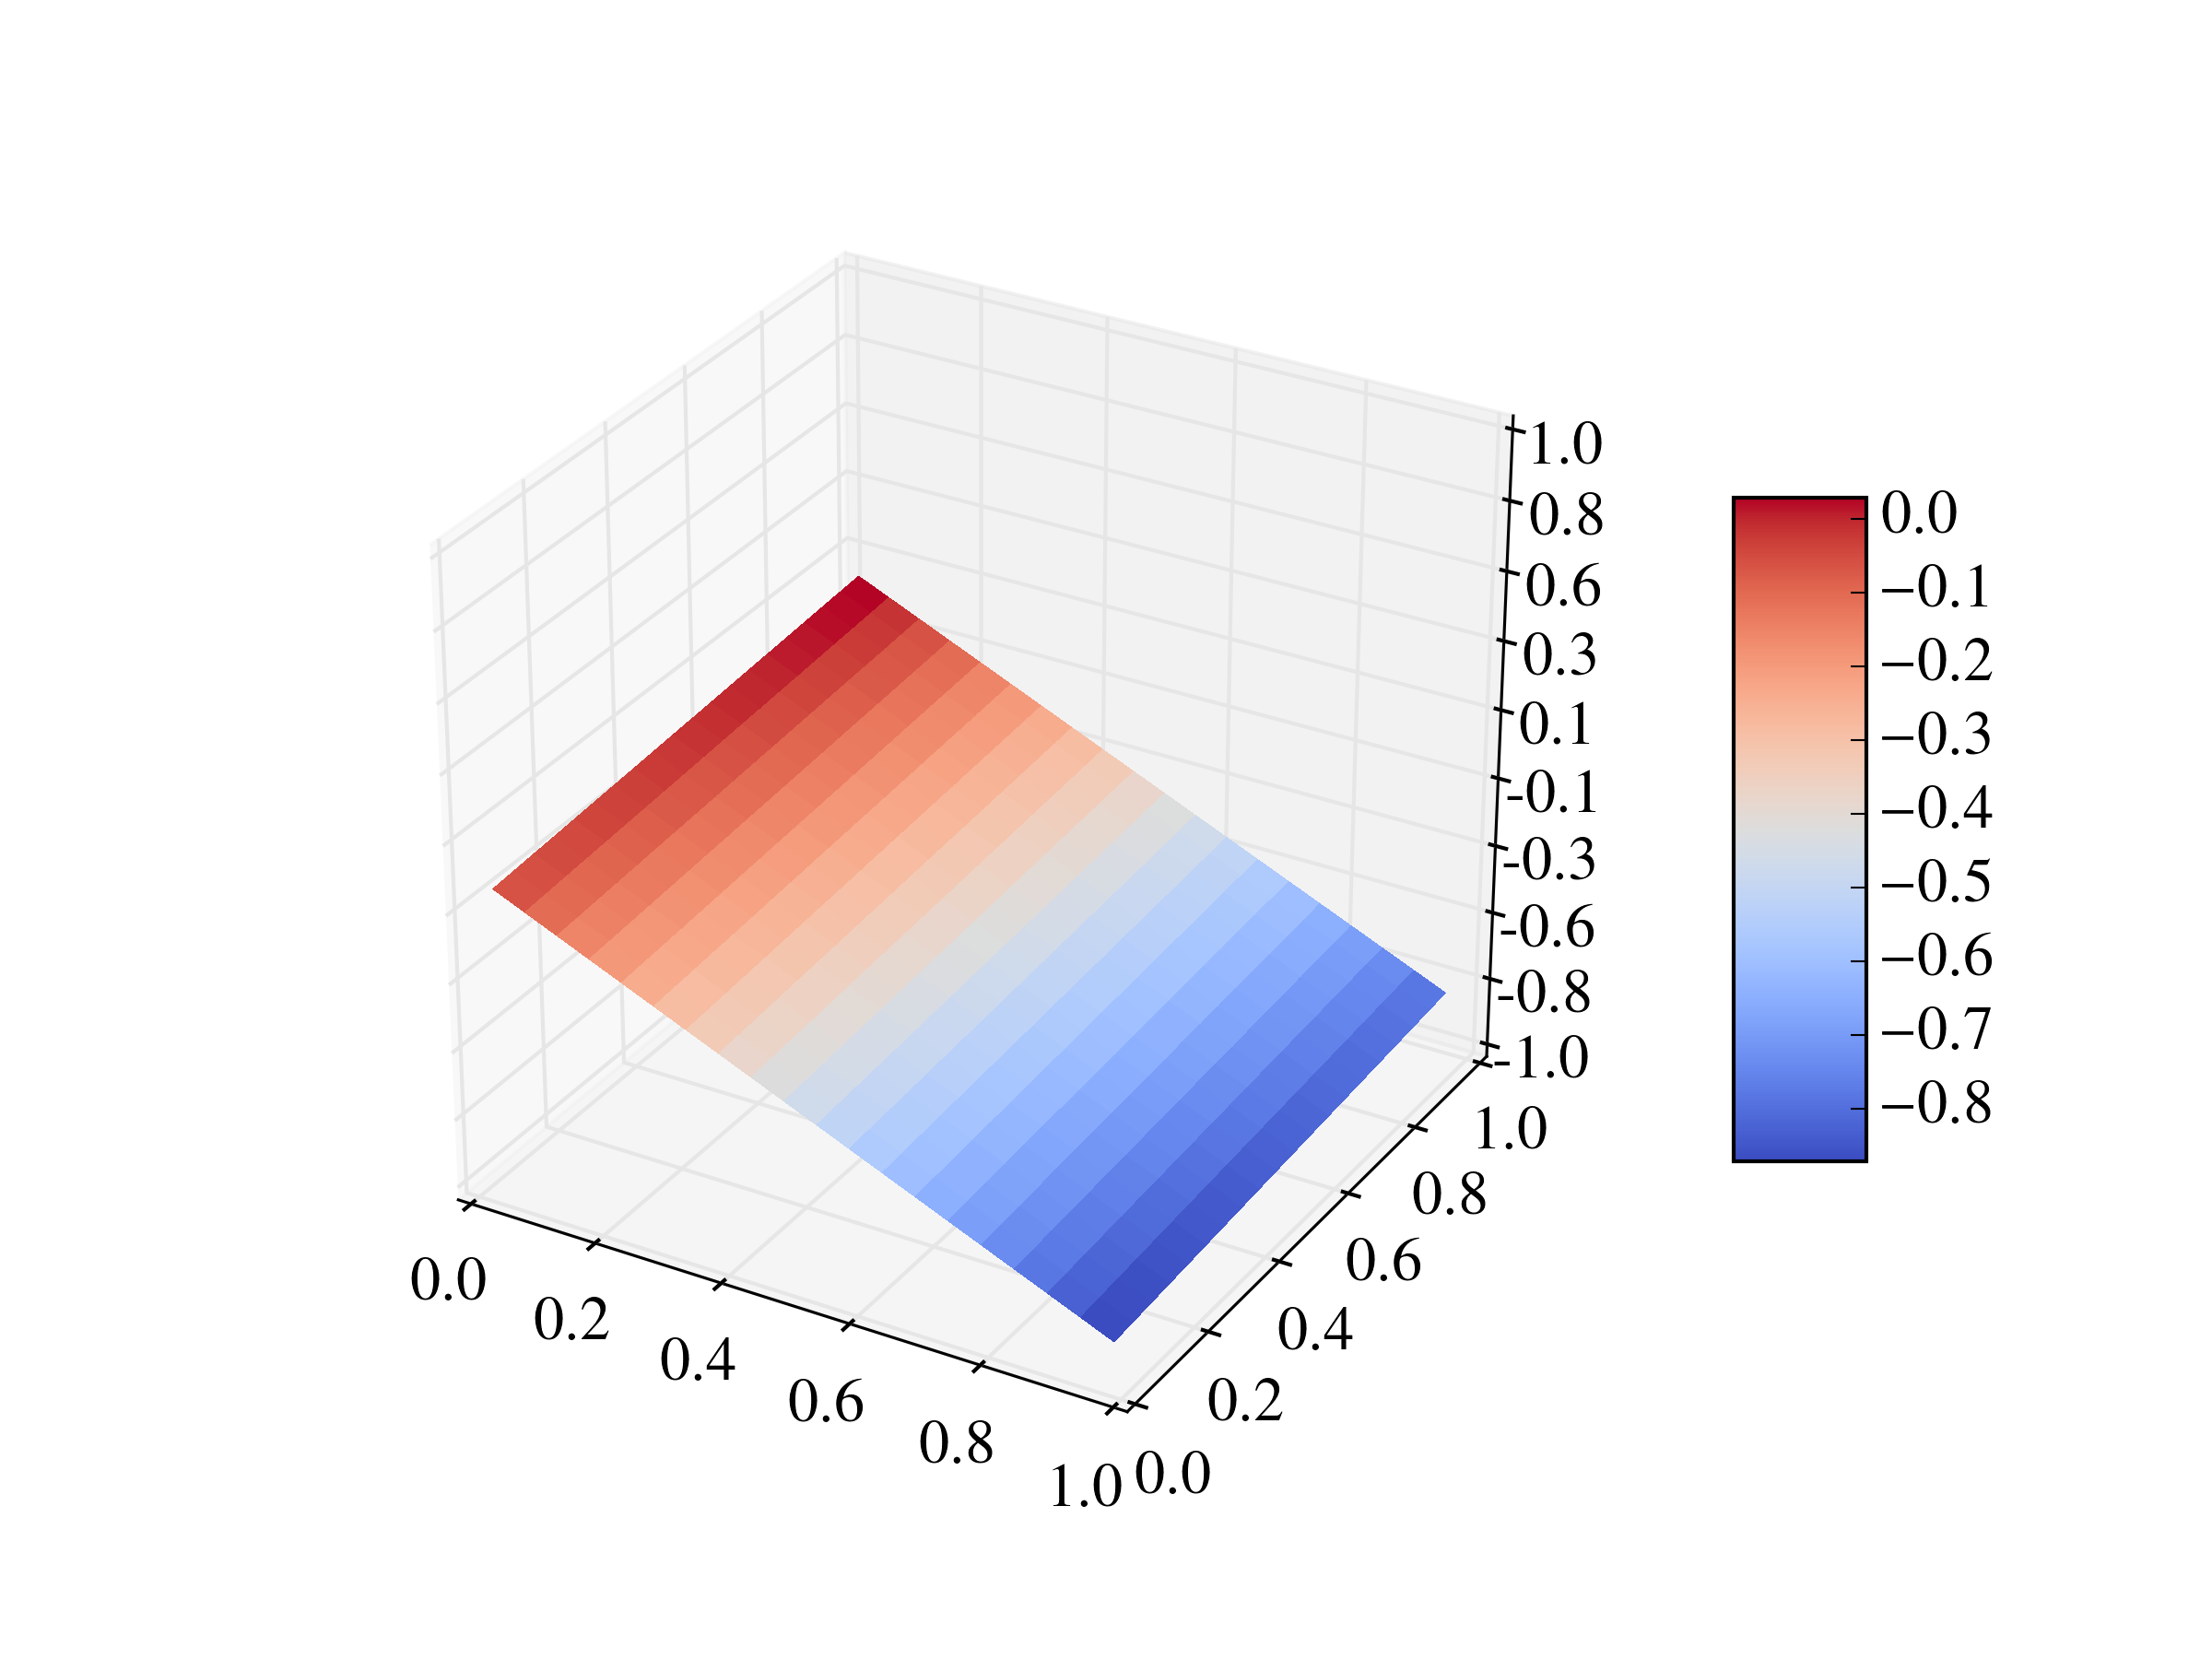
\includegraphics[width=10cm]{img/phiProblem2.png}
\caption{Função potencial $\phi$\label{p33}}
\end{figure}
\newpage

\subsection{$\mathbf{M} = x\mathbf{i}-y\mathbf{j}$ e $\mathbf{H} = \mathbf{i}+\mathbf{j}$}
\paragraph{} Veja Figuras \ref{p41}, \ref{p42} e \ref{p43}. Para este caso, tem-se: $\max \frac{1}{\mu_0}\nabla\cdot \mathbf{B}  = 1.82\cdot 10^{-12}$ e $\max \nabla\times \mathbf{H}  =4.95\cdot 	10^{-13}$

\begin{figure}[!ht]
\centering
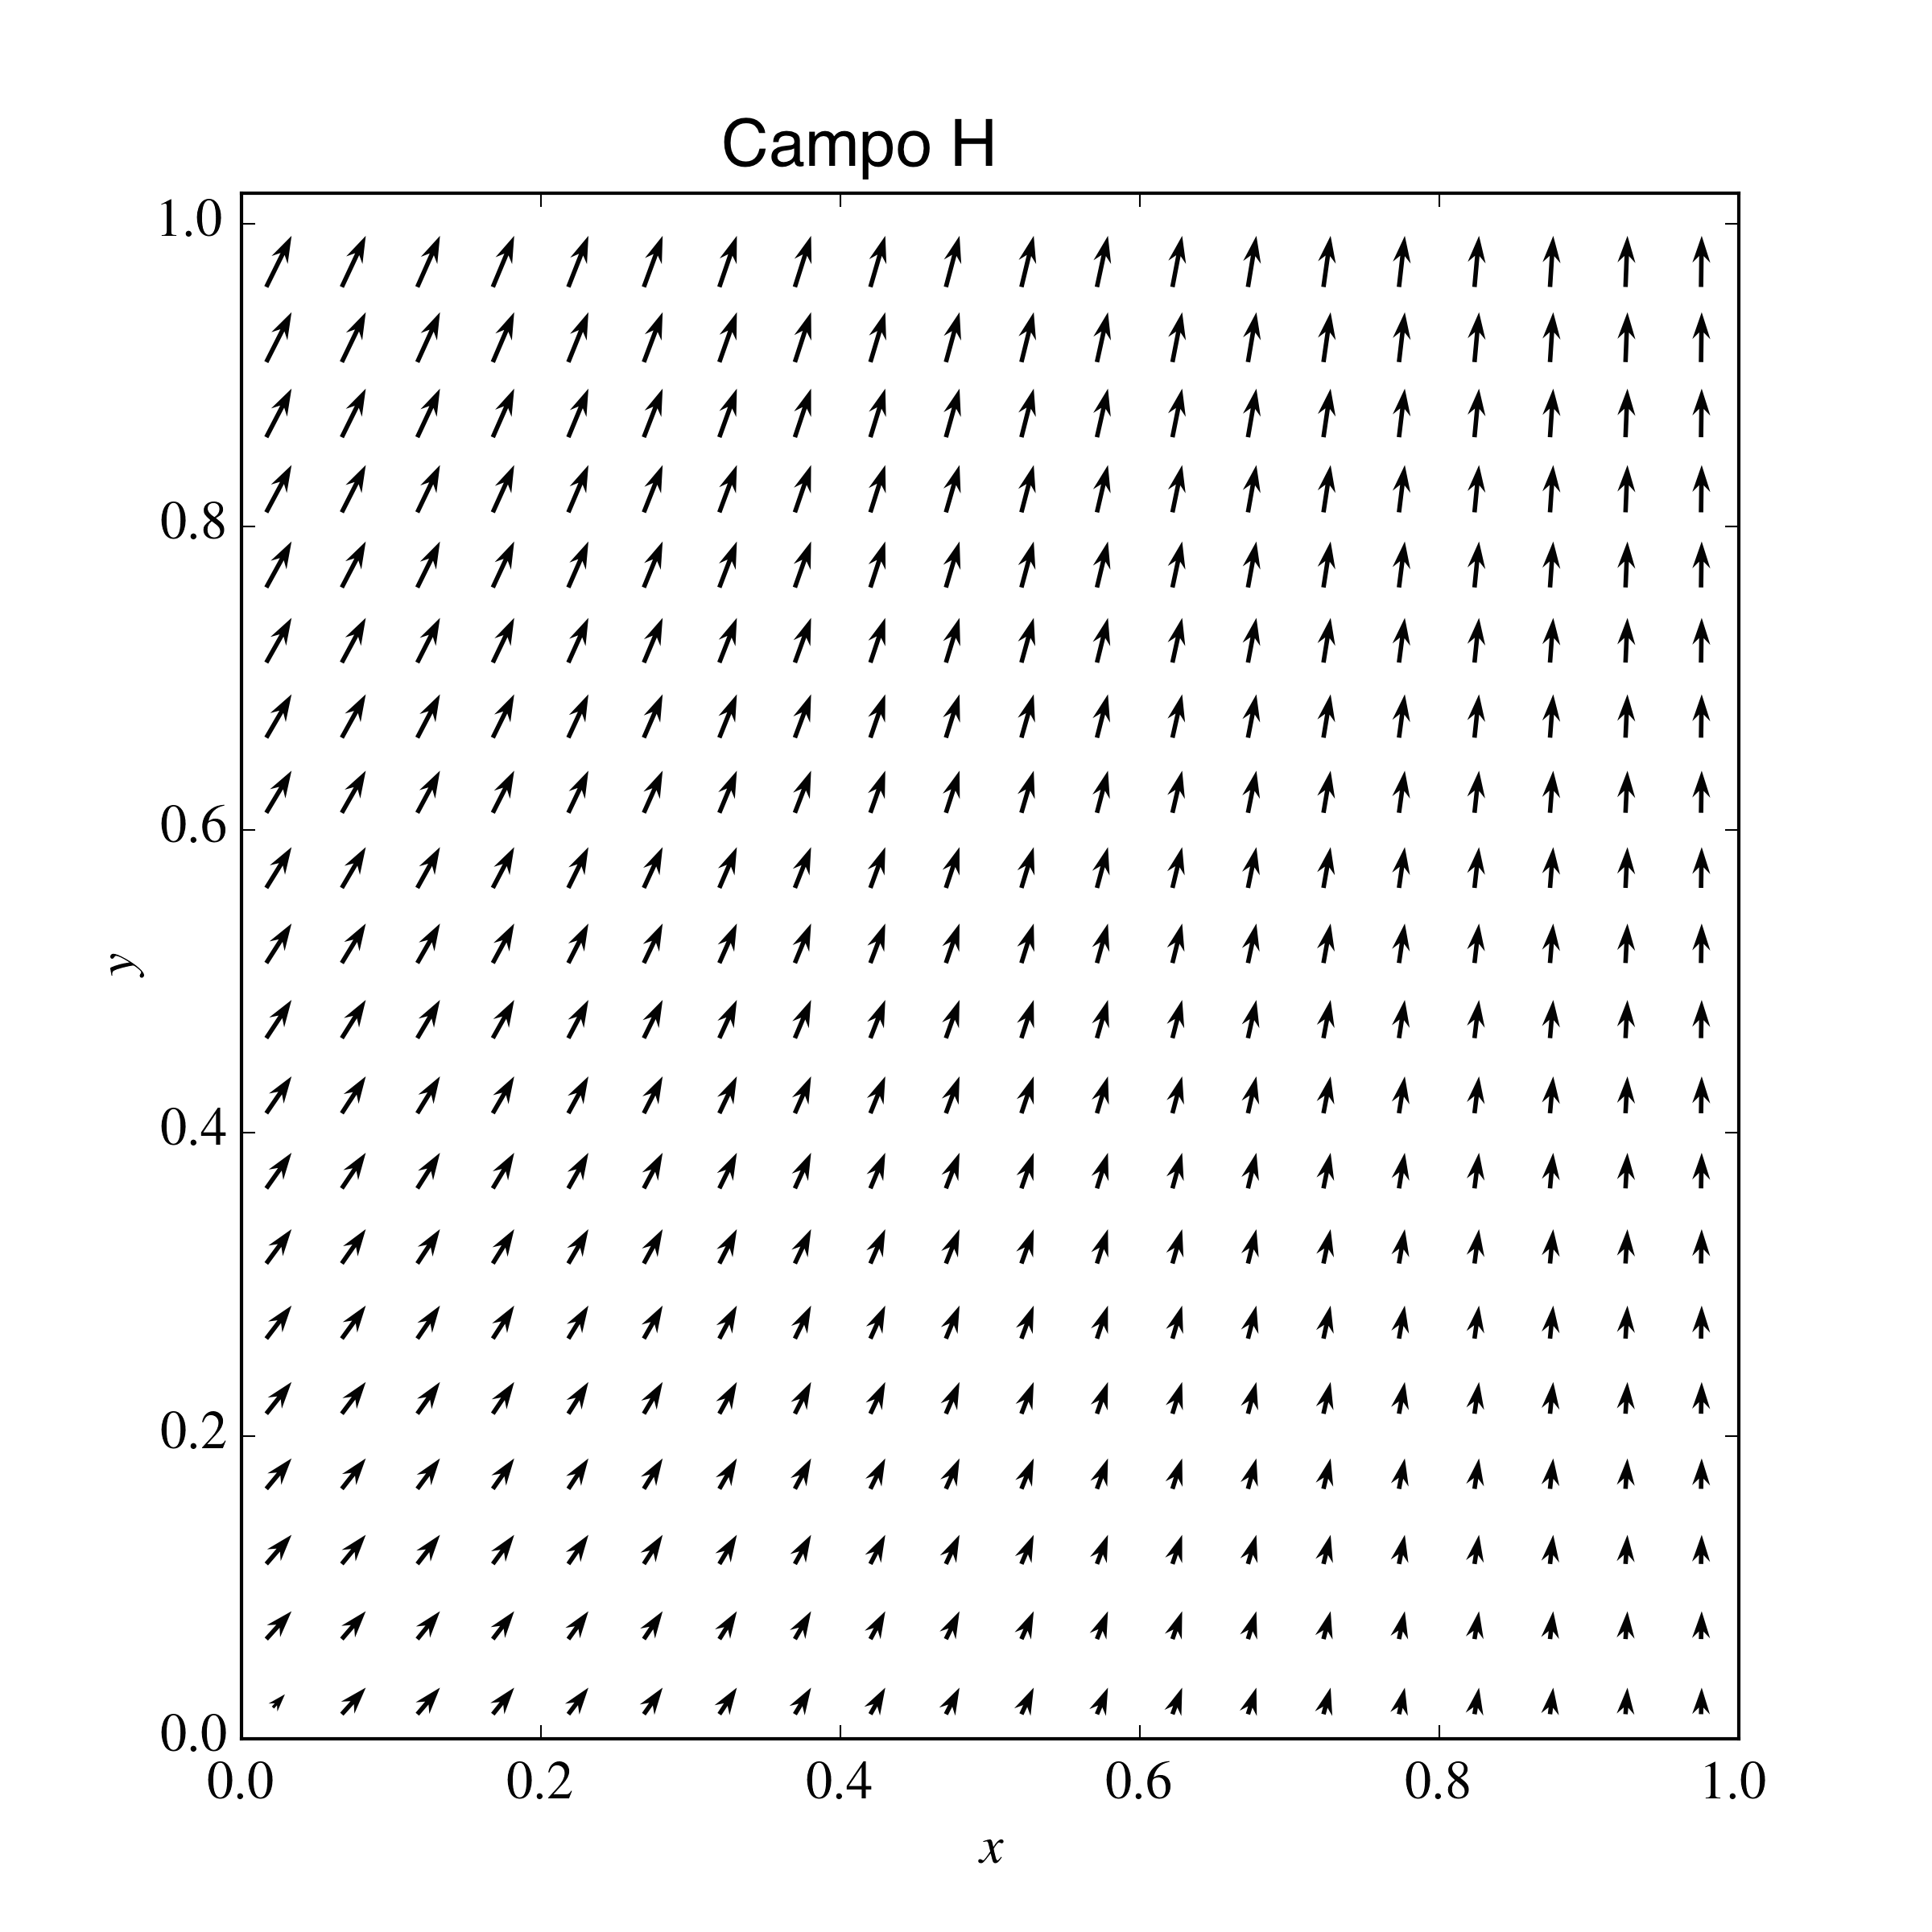
\includegraphics[width=10cm]{img/Hproblem3.png}
\caption{Campo vetorial $\mathbf{H}$ dentro da cavidade\label{p41}}
\end{figure}

\begin{figure}[!ht]
\centering
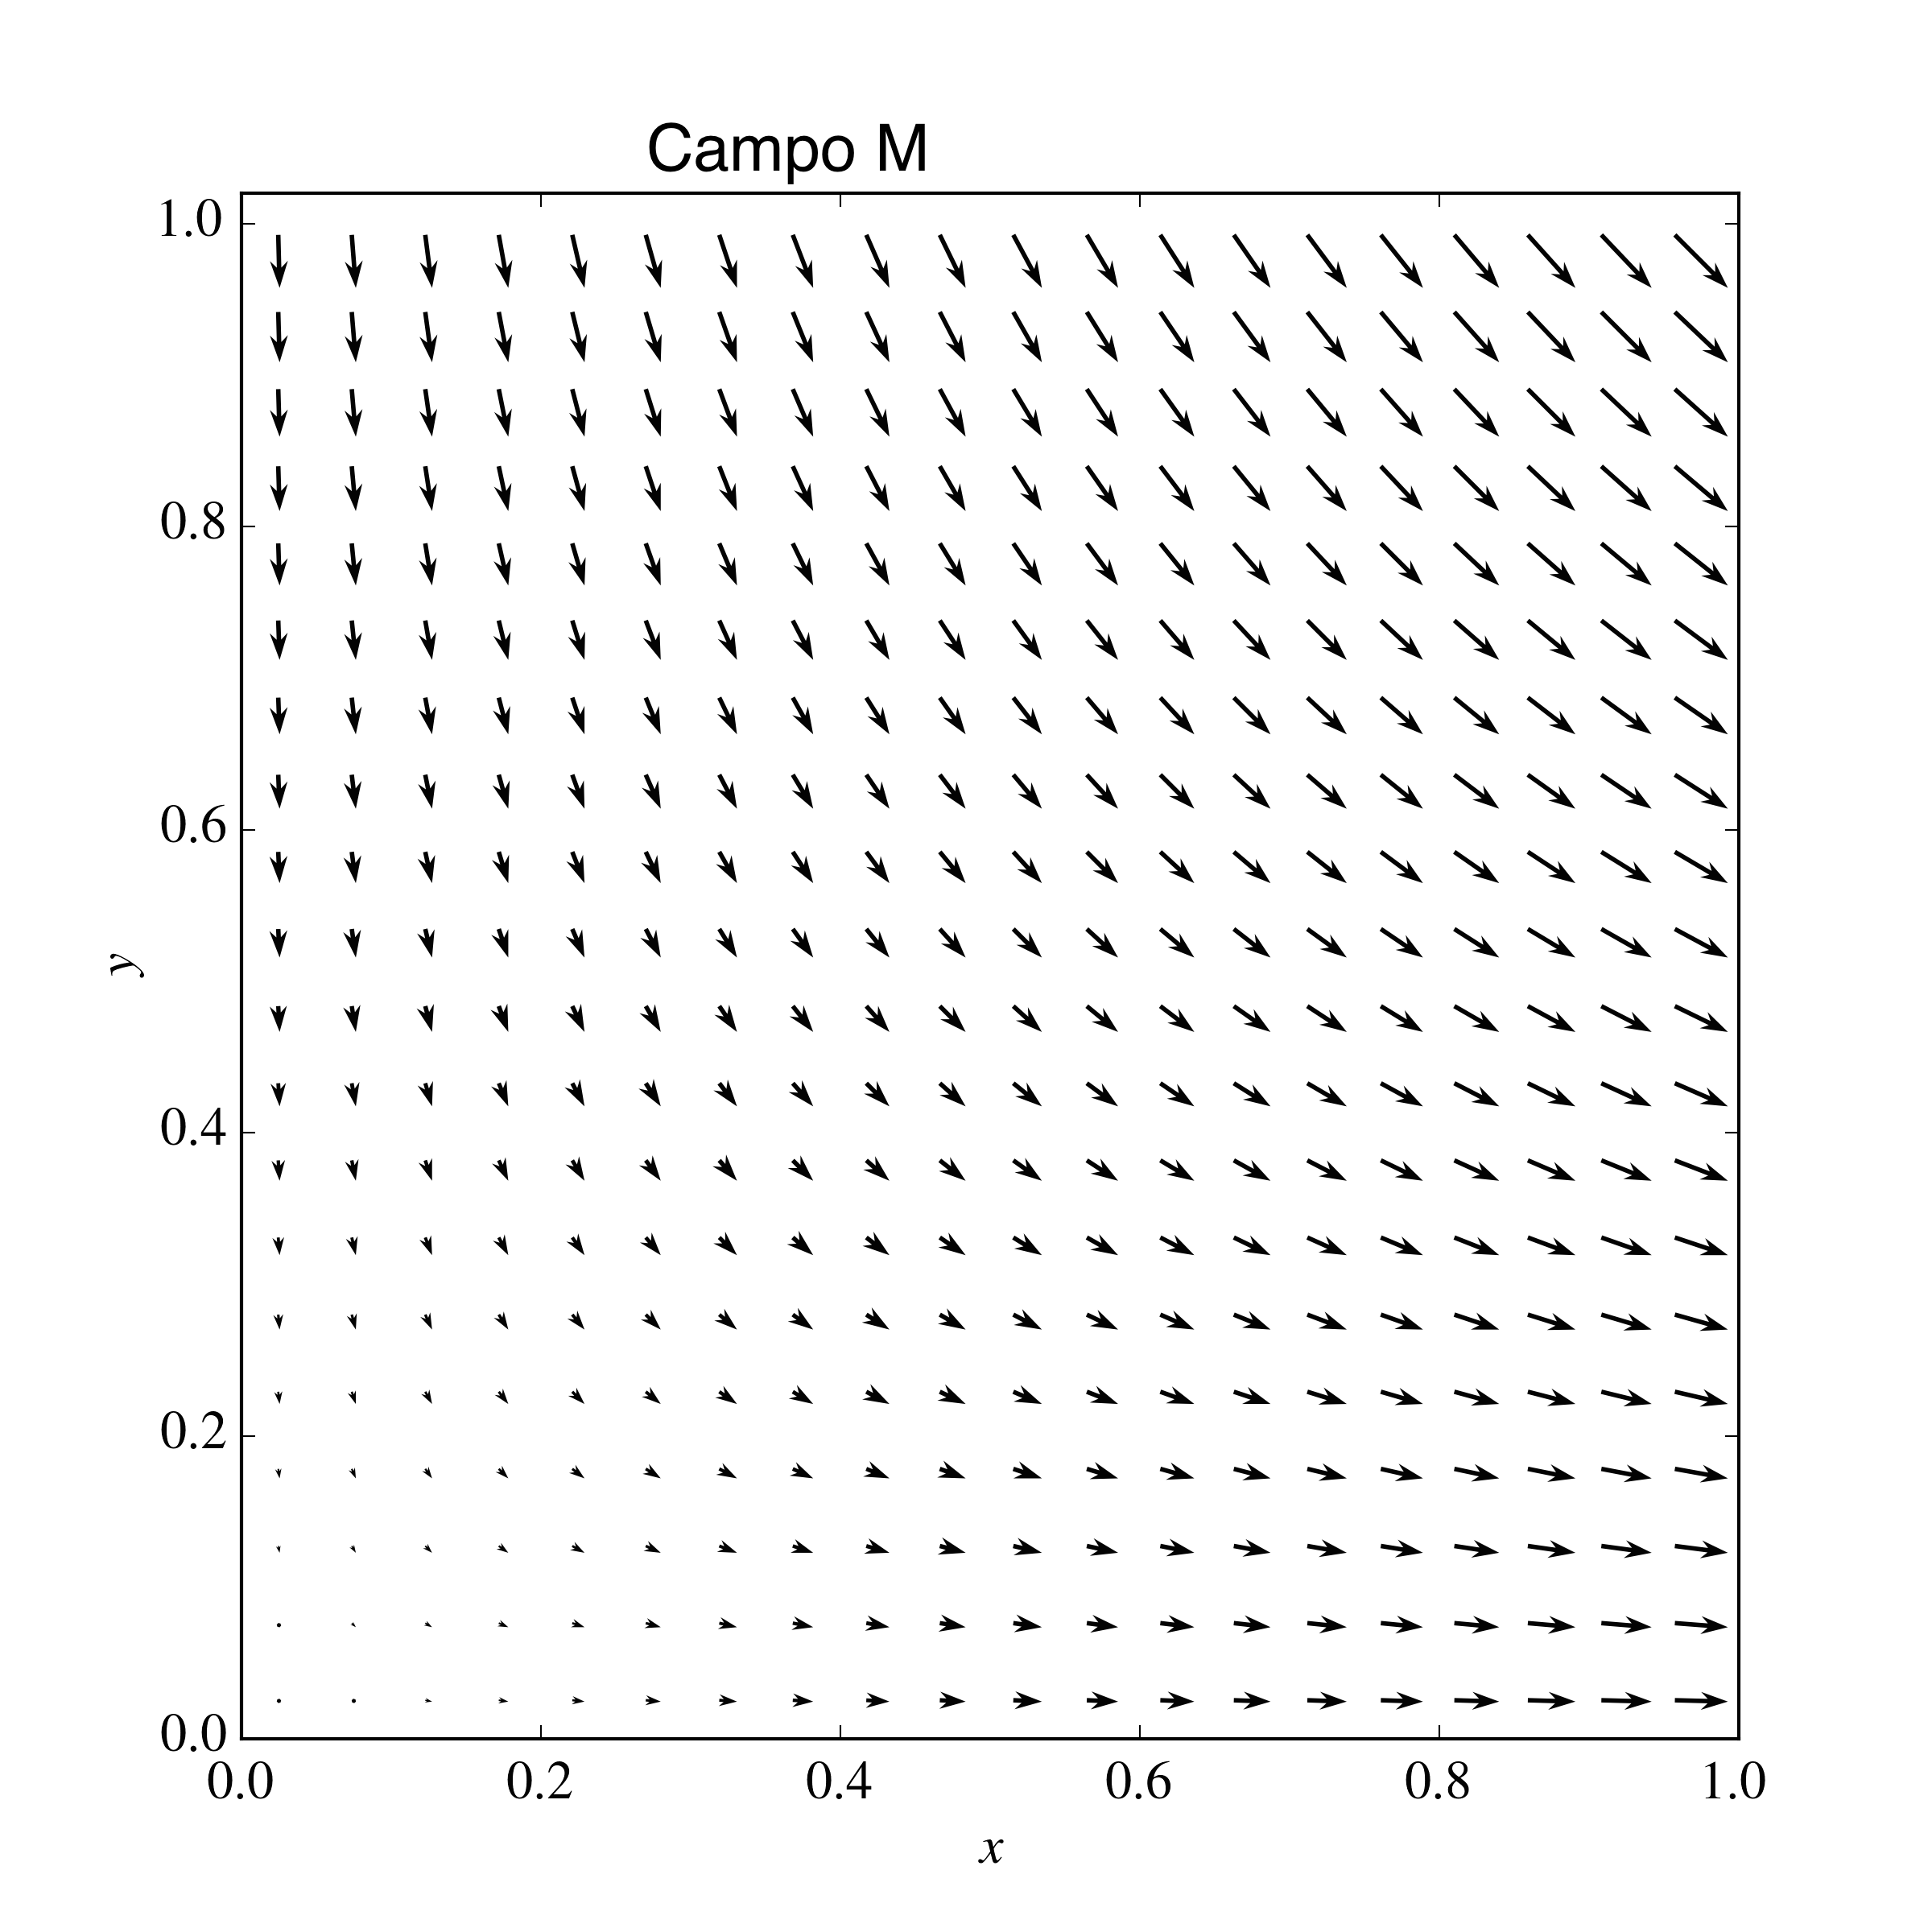
\includegraphics[width=10cm]{img/Mproblem3.png}
\caption{Campo vetorial $\mathbf{M}$ dentro da cavidade\label{p42}}
\end{figure}

\begin{figure}[!ht]
\centering
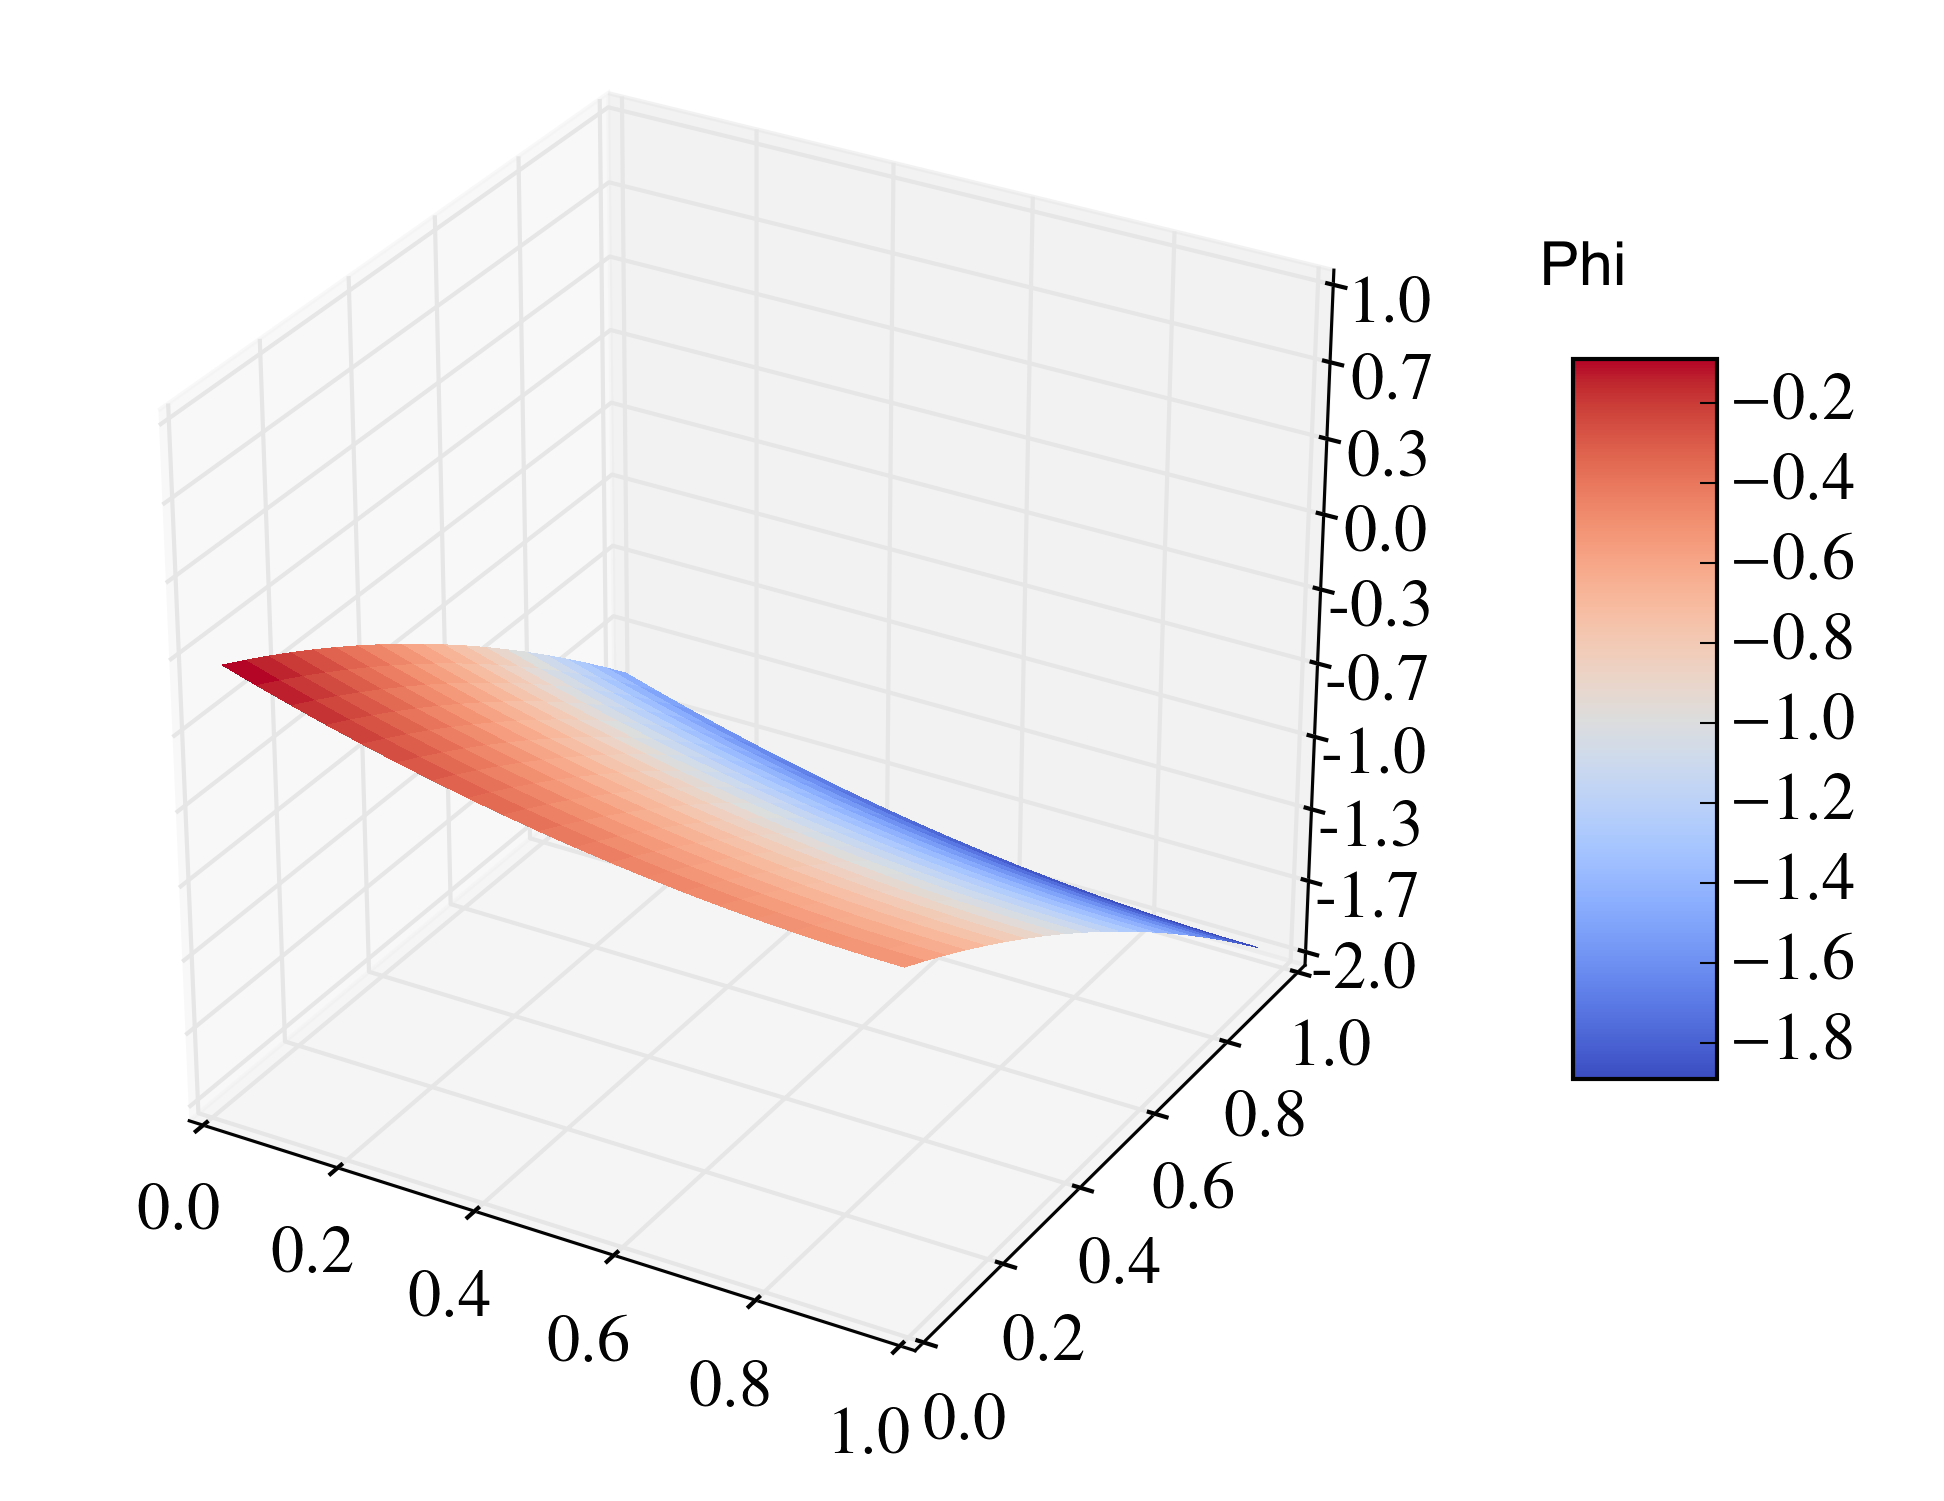
\includegraphics[width=10cm]{img/phiProblem3.png}
\caption{Função potencial $\phi$\label{p43}}
\end{figure}

\end{document}
